% Root File for a UCSB Dissertation
%
%
% draft options
%\documentclass[12pt,twoside,draft]{ucthesis}
% final options: 
\documentclass[12pt,oneside,final]{ucthesis}

\usepackage{graphics,epsfig}
\usepackage{pgfplots}
\usepackage{pgfplotstable}
\usepackage{sansmath}
\usepackage{mathptmx}
\usepackage{subfigure}
\usepackage{multirow}
\usepackage{breqn}
\usepackage{rotating}
%\usepackage{amssymb, amsmath, amsfonts, epsfig, graphicx, graphics, latexsym, makeidx, psfig, subeqn, verbatim, xspace,textco
%mp}
\pgfplotsset{
    %You are supposed to use append style rather than just setting
    %parameters globally so they are easier to override to special cases
    %thickness options:thin,ultra thin,very thin,semithick,thick,very thick
    every axis/.append style={
        thick,
        tick style={thick},
        tick label style={font=\small\mathversion{sans}\sffamily},
        label style={font=\small\sffamily},
        font={\small\sffamily},
        mark size=1.0
    },
    every legend/.append style={font={\small\mathversion{sans}\sffamily}}
}
\pgfplotsset{
    every mark/.append style={solid}
}
\pgfplotscreateplotcyclelist{mcolor}{%
    {blue,every mark/.append style={fill=blue},mark=*},
    {red,every mark/.append style={fill=red},mark=square*},
    {brown,every mark/.append style={fill=brown},mark=triangle*,mark size=1.5},
    {black,every mark/.append style={fill=black},mark=diamond*,mark size=1.5},
    {green!60!black,every mark/.append style={fill=green!60!black},mark=pentagon*,mark size=1.4},
    {magenta!90!black,every mark/.append style={fill=magenta!90!black},mark=star,mark size=1.5},
    {densely dashed,blue,every mark/.append style={fill=blue},mark=*},
    {densely dashed,red,every mark/.append style={fill=red},mark=square*},
    {densely dashed,brown,every mark/.append style={fill=brown},mark=triangle*,mark size=1.5},
    {densely dashed,black,every mark/.append style={fill=black},mark=diamond*,mark size=1.5},
    {densely dashed,green!60!black,every mark/.append style={fill=green!60!black},mark=pentagon*,mark size=1.4},
    {densely dashed,magenta!90!black,every mark/.append style={fill=magenta!90!black},mark=star,mark size=1.5}}

\pgfplotscreateplotcyclelist{mmark*}{
    {mark=*},
    {mark=square*},
    {mark=triangle*,mark size=1.5},
    {mark=diamond*,mark size=1.5},
    {mark=pentagon*,mark size=1.4},
    {mark=star,mark size=1.5},
    {mark=asterisk,mark size=1.5},
    {mark=+,mark size=1.5},
    {mark=Mercedes star,mark size=1.5}}

\pgfplotscreateplotcyclelist{mline}{
    {solid,blue,every mark/.append style={fill=blue}},
    {densely dashed,red,every mark/.append style={fill=red}},
    {densely dotted,brown,every mark/.append style={fill=brown}},
    {loosely dotted,black,every mark/.append style={fill=black}},
    {loosely dashed,green!60!black,every mark/.append style={fill=green!60!black}},
    {densely dashdotted,magenta!90!black,every mark/.append style={fill=magenta!90!black}},
    {densely dashdotdotted,teal,every mark/.append style={fill=teal}},
    {loosely dashdotted,orange,every mark/.append style={fill=orange}},
    {loosely dashdotdotted,violet,every mark/.append style={fill=violet}}}

    \pgfplotsset{cycle list name=mcolor}

\newcommand{\comments}[1]{}
%% Document Parts

% run latex with only these files; it's faster without all eps figures etc.
%\includeonly{Title,Front,Intro}
%\includeonly{Title,Front,Intro,Literature,Chapter1,Chapter2,Conclusions}

%%% Document Portion:

\begin{document}

%% Front Matter:
%%%%%%%%%%%%%%%%%%%%%%%%%%%
% TITLE PAGE INFORMATION %
%%%%%%%%%%%%%%%%%%%%%%%%%%%

\title{Collocated Data Deduplication for Virtual Machine Backup in the Cloud}

%\germantitle{Der Tolle Deutsche Titel}

\author{Wei Zhang}

%%%%%%%%%%%%%%%%%%%%%%%%%%%%%%%%%%
% DECLARATIONS FOR FRONT MATTER %
%%%%%%%%%%%%%%%%%%%%%%%%%%%%%%%%%%
\report{Dissertation}
\degree{Doctor of Philosophy}
\degreemonth{January}
\degreeyear{2014}
\approvalmonth{January}
\approvalyear{2014}

\chair{Professor Tao Yang}
\committeeII{Professor Jianwen Su}
\committeeIII{Professor Rich Wolski}
\nummembers{3}

\field{Computer Science}
\campus{Santa Barbara}
          % First Page
\maketitle             % Make Title Page

\begin{frontmatter}
\approvalpage
\copyrightpage
\begin{dedication}
   \null\vfil{%\large

\hspace{\stretch{1}} 
\begin{minipage}{3.2in}
\begin{center}
To my family.
\end{center}
\end{minipage}

} \vfil\null
\end{dedication}
\begin{acknowledgements}
\addcontentsline{toc}{chapter}{Acknowledgements}

First of all, I want to take this opportunity to thank my advisor Professor Tao Yang for 
his invaluable advice and instructions to me on selecting interesting and challenging
research topics, identifying specific problems for each research phase, 
as well as preparing for my future career. I would also like to thank my committee
members, Professor Rich Wolski and Professor Jianwen Su, for their pertinent and helpful
instructions on my research work. 

I also want to thank members and ex-members of my research group, Michael Agun, Gautham Narayanasamy,
Prakash Chandrasekaran, Xiaofei Du, and Hong Tang, 
for their incessant support in the forms of technical discussion, 
system co-development, cluster administration, and other research activities.

I owe my deepest gratitude to my parents, for their love and support, which give 
me the confidence and energy to overcome all past, current, and future difficulties. 

Finally and most importantly, I would like to express my gratitude beyond 
words to my wife, Jiayin, who has been encouraging and inspiring me 
since we met in love. We went through all the difficlut times together,
and depended on each other in this foreign place one Pacific Ocean away from our homeland.
Every step forward I have made is unimaginable without Jiayin's support.

This dissertation study was supported in part by NSF IIS-1118106.
\end{acknowledgements}

\begin{vitae}
\addcontentsline{toc}{chapter}{Curriculum Vit\ae}
{\small

\begin{vitaesection}{Education}
\vspace{-0.1cm}
   \item [2002 -- 2005] Master of Science in Computer Science, Tsinghua University, Beijing, China.
    
   \item [1997 -- 2001] Bachelor of Science in Electrical Engineering, Wuhan University, Wuhan, China.

\end{vitaesection}

% \begin{vitaesection}{Experience}
% \vspace{-0.1cm}
%    \item [1999 -- 2000] Graduate Research Assistant, University of California,
%     Santa Barbara.

% \end{vitaesection}

%{\bf Selected Publications}
\begin{vitaesection}{Publications}
%\vspace{-0.5cm}
\item Michael Daniel Agun, Tao Yang, Wei Zhang. ``Asynchronous Source-side Deduplication for Cloud Data Backup''. {\it To be submitted for publication}.

\item Wei Zhang, Michael Daniel Agun, Tao Yang, Hong Tang. ``VM-Centric Snapshot Deduplication for Converged Cloud Architectures''. {\it Submitted to 2014 ACM Symposium on Cloud Computing (SoCC'14)}.

\item Wei Zhang, Tao Yang, Gautham Narayanasamy, Hong Tang. ``Low-Cost Data Deduplication for Virtual Machine Backup in Cloud Storage''. {\it In Proceedings of the 5th USENIX Workshop on Hot Topics in File and Storage Technologies (HotStorage'13)}, July 2013.

\item Wei Zhang, Hong Tang, Hao Jiang, Tao Yang, Xiaogang Li, Yue Zeng. ``Multi-level Selective Deduplication for VM Snapshots in Cloud Storage''. {\it In Proceedings of the 5th IEEE International Conference on Cloud Computing (CLOUD'12)}, June 2012.

\item Wen Ye, Wei Zhang, Rich Wolski. ``Simulation-Based Augmented Reality for Sensor Network Development''. {\it In Proceedings of the 5th ACM Conference on Embedded Networked Sensor Systems (SenSys'07)}, November 2007.

\item Wei Zhang, Haoxiang Lin. ``A Versatile Cryptographic File System for Linux''. {\it In Journal of Micro Computer Systems, China}, 2006.

\item Wei Zhang, Fuchun Sun. ``An Improved FCM Algorithm Based On Search Space Smoothing''. {\it In Proceedings of the 1st IASTED International Conference on Computational Intelligence (CI'05)}, July 2005.

\vspace{0.3cm}


\end{vitaesection}

}

\end{vitae}

%\input{Preface}
%
%  Abstract
%

\begin{abstract}

\addcontentsline{toc}{chapter}{Abstract}
Cloud platforms that host a large number of virtual machines (VMs) have high storage demand for frequent backups
of VM snapshots. Content signature based deduplication is necessary to eliminate excessive redundant blocks.
While dedicated backup storage systems can be used to reduce data  redundancy,
such an architecture is expensive and introduces huge network  traffic in a large cluster.
This thesis research is focused on a low-cost backup and deduplication service collocated with
other cloud services to reduce infrastructure and network cost.

The previous research for cluster-based data deduplication has concentrated on various inline solutions.
The first part of the thesis work is a  highly parallel and offline solution with synchronized backup scalable
for a large number of virtual machines. The key idea is to separate duplicate detection from the actual storage backup,
and to partition global index and detection requests among machines using fingerprint values.
Then each machine conducts duplicate detection partition by partition independently with minimal memory consumption.
Another optimization is to allocate and control buffer space for exchanging detection requests and duplicate summaries
among machines. The resource requirement in terms of memory and disk usage for the proposed solution is
very small while the backup efficiency in terms of overall throughput and time is not compromised.
Our evaluation validates this and shows a satisfactory backup throughput in a large cloud setting.

The second part of the thesis work is a VM-centric collocated backup service with inline deduplication.
The key difference compared to the previous work is its novelty in fault resilience and low resource usage.
We propose a multi-level selective deduplication scheme which integrates similarity-guided and
popularity-guided duplicate elimination under a stringent resource requirement.
This scheme uses popular common data to facilitate fingerprint comparison, localizes deduplication
as much as possible within each VM, and associates underlying file blocks with one VM for most of cases.
The main advantage of this scheme is that it strikes a balance between inner and inter VM deduplication,
increasing parallelism and  improving reliability.  Our analysis shows that this VM-centric scheme can provide
better fault tolerance while using a small amount of computing and storage resource.
We have conducted a comparative evaluation of this scheme on its competitiveness in terms of deduplication efficiency and backup throughput.

\abstractsignature

\end{abstract}


\tableofcontents
\listoffigures
\listoftables
\end{frontmatter}


% the chapters

% spacing in figures and tables and their captions can be
% changed here (\ssp for single-space, empty for same as surrounding 
% text); for this to work, the command \figsp has to be included
% in every figure and table right after the \begin{figure}
\def\figsp{\ssp}
%\def\figsp{}


\chapter{Introduction}
\label{chap:intro}
\section{Problem Statement and Motivation}
\label{intro:prob}
The ubiquity of the cloud computing has resulted in the 
widespread availability of cluster-based services and applications accessible through
the Internet. Examples include online storage services, big data analytics, and e-commerce websites.
In such a cluster-based cloud environment,
each physical machine runs a number of virtual machines as  instances of a guest operating system
to contain different kind of user applications,
and their data is stored in virtual hard disks which are represented
as virtual disk image files in the host operating system.
Frequent snapshot backup of virtual disk images is critical to increase  the service reliability
and protect data safety.
For example, the Aliyun cloud, which is  the largest cloud service provider by Alibaba in China,
automatically conducts  the backup of virtual disk images to all active users every day.

The cost of supporting a large number of concurrent backup streams is high
because of the huge storage demand.
If such VM snapshot data is plainly backed up without any duplicate reduction, storage waste would be
extreme high. For example, a fresh Windows server 2008 installation costs 25 GB on the virtual disk,
and they are almost certainly duplicated with other Windows VM instances\cite{common07, pedal96}.
Using a separate  backup service with full deduplication support~\cite{venti02,bottleneck08}
can effectively identify and remove content duplicates among snapshots,
but such a solution can be expensive. There is also a large amount of
network traffic to transfer  data from the host machines to the backup facility
before duplicates are removed.

Unlike the previous work dealing with general file-level
backup and deduplication inside a centralized storage appliance, our research is focused on virtual
disk image backup in a cluster of machines. Although we treat each virtual disk as a
file logically, its size is very large. On the other hand, we need
to support parallel backup of a large number of virtual disks
in a cloud every day. One key requirement we face at a busy cloud cluster
 is that VM snapshot backup should only use a minimal
amount of system resources so that most of resources is kept
for regular cloud system services or applications. Thus our
objective is to exploit the characteristics of VM snapshot data
and pursue a cost-effective deduplication solution. Another
goal is to decentralize VM snapshot backup and localize
deduplication as much as possible, which brings the benefits
for increased parallelism and fault isolation.

Despite its importance, storage deduplication remains a challenging task for cloud storage providers,
especially for resource-constrained large-scale public VM clouds.
In recognizing this importance and
the associated challenges,  my thesis is that

\textit{It  is  possible  to  build  an efficient, scalable, and fault-tolerant backup service
supporting highly accurate deduplication with sustainable high throughput.}

In  other  words,  the  main  goal  of this  study  is  to  answer  the  following
question.  Given a large scale VM cluster running tens of thousand of VMs,
how can such a snapshot backup service identify whether a piece of data in VM disk
really needs a backup? And how to manage backup data under complex sharing relationship?
This dissertation investigates
techniques  in  building  a snapshot storage architecture that provides
low-cost deduplication support for large VM clouds.  In particular,  it
contains the following contributions to establish my thesis:

\begin{itemize}
\item The design of a low-cost multi-stage parallel deduplication solution for automatically batched deduplication.
\item An inline multi-level deduplication scheme with similarity-guided local detection and
popularity-guided global detection.
\item The development and analysis of a VM-centric storage approach which considers fault isolation and integrates multiple duplicate detection strategies.
\item Fast and efficient garbage collection with approximate snapshot deletion and leak repair.
\end{itemize}

In general, this  dissertation  study  is  built  upon  a  large  body  of previous  research
in storage deduplication and distributed storage systems.  The goal
of this work is to provide low-cost deduplication support and storage management for
large-scale resource-constrained VM clouds. This solution should be collocated with existing
cloud infrastructure services and require no dedicated hardware support. It also needs to
accomplish good deduplication efficiency and does not comprise the data reliability due to the
inherent volatility of commodity hardware.
Under the  above consideration, our system is designed to support multiple levels of deduplication
depending on backup requirements. The objective is to provide satisfactory deduplication efficiency
and high throughput with the emphasis on low resource usage and fault tolerance.

\section{Dissertation Organization}
\label{intro:organ}
The rest of this dissertation is organized as follows.
Chapter~\ref{chap:back} gives the background of thesis problems.
Chapter~\ref{chap:overview} presents the overall VM snapshot storage architecture.
Chapter~\ref{chap:offline}  describes a synchronous and parallel deduplication scheme for batched complete deduplication.
Chapter~\ref{chap:inline} studies a multi-level selective deduplication solution for inline deduplication.
Chapter~\ref{chap:data}  describes a VM-centric storage management with approximate deletion.
Chapter~\ref{chap:concl}  concludes this  dissertation  and  briefly discusses some potential future work.


\chapter{Background}
\label{chap:back}
At a cloud cluster node, each instance of a guest operating system runs on a virtual machine, accessing virtual hard disks 
represented as virtual disk image files in the host operating system.
For VM snapshot backup, file-level semantics are normally not provided.
Snapshot operations take place at the virtual device driver level, which
means no fine-grained file system metadata can be used to determine the changed data. 
Backup systems have been developed to use content fingerprints to identify duplicate
content~\cite{venti02,Rhea2008}.  

Many deduplication systems have been built for VM backup purposes. 
In this chapter we will investigate several system design options at high-level.
Section~\ref{back:coll} discusses the comparison of collocated solution vesus dedicated appliance.
Section~\ref{back:trade} talks the tradeoffs in designing a deduplication storage system.
Section~\ref{back:algo} introduces deduplication optimizations.

\section{Architecture Options - Collocated vesus Dedicated} 
\label{back:coll}
Dedicated deduplication is a great way to augment existing tape based backup infrastructures due to its simple integration with existing backup applications. So if an end user is happy with their current backup application, a Dedicated approach may be very compelling as it does not necessitate a significant change of the backup infrastructure or the relearning of a new backup application.

One of the strongest use cases for Dedicated deduplication is protecting large Oracle or SQL database (in excess of 2TBs) environments. Since each of these applications can natively backup their data to a Dedicated appliance, from an integration standpoint, there is low/no barrier to entry to begin protecting these environments rapidly. Some deduplication appliance manufacturers even offer direct integration with database backup tools like Oracle RMAN. This helps drive out some of the inefficiencies in the data center as both backup administrators and DBAs can share a common pool of backup resources and achieve reductions where there may be an overlap in backup processes.

Another benefit to database target deduplication is a reduction in the consumption of primary storage resources. Many DBAs utilize a disk to disk to tape backup scheme to protect log files, table spaces etc. on primary storage that has no deduplication capability. Between periodic snapshots and direct dumps to disk, there tends to be an over consumption of expensive disk resources when protecting database environments. By migrating database backups to a deduplication appliance, scarce primary storage resources can be reclaimed for production applications. Whats more, the deduplication effect for database environments can range from a 5-1 to a 20-1 reduction in the physical disk or tape space required to perform normal backup operations - potentially generating a return on investment.

In short, Dedicated deduplication provides an easy entry point for customers interested in leveraging the efficiencies of deduplication to reduce backup windows, enhance data protection and improve overall operational efficiencies in the data center without making major changes to their environment. 

Collocated deduplication generally consists of backup application software with embedded deduplication at the client layer and some form of disk storage to serve as the repository for backup data. As the name implies, Collocated data deduplication takes place at the source or where data originates - at the server or application layer. Collocated deduplication offerings consist of placing a lightweight backup agent at the virtual or physical server and then only backing up the unique data segments that have changed since the prior backup job. The data segments are then sent over the LAN and/or WAN to a disk based storage grid for protection.

The advantages of Collocated deduplication are rapid backup windows and a large reduction in the volume of LAN/WAN traffic generated during the backup window. Instead of pushing a full backup over the wire from a media server each night, unique deduplicated backup segments trickle between the application hosts and the backend deduplication storage grid. The data transfers are extremely efficient - equivalent to a meta-data handshake. Think speed of source side deduplication as an incremental (only more efficient) forever with the benefit of producing a full backup each night.

In general, Collocated deduplication is a great solution for environments with a low daily data change rate. Great use cases for Collocated deduplication solutions include data on the edge  remote offices and laptops in the field (great for C level execs) and file heavy environments (NAS, VMware). In the case of remote offices, often the investment in Collocated deduplication can be justified by the cost avoidance attained by eliminating the legacy remote office backup infrastructure  backup server hardware, software, tape libraries, tape media, courier expenses, etc.

In the VM snapshot backup case that we study, there is hardly any value for deploying dedicated backup
solution because it's not affordable to VM users. Therefore we seek for low-cost collocated deduplication options
to reduce the VM snapshot storage cost.
Collocating a backup service on the existing
cloud cluster avoids the extra cost to acquire a dedicated backup facility
and reduces the network bandwidth consumption in transferring the
raw data for backup. 

\section{Tradeoff in Design Goals}
\label{back:trade}
Given we are designing scalable low-cost collocated deduplication solutions,
the effectiveness of a deduplication system is determined 
by the extent to which it can achieve three mutually competing goals: 
deduplication efficiency, throughput, and job turnaround time. 
Deduplication efficiency refers to
how well the system can detect and share duplicate data
units which is its primary compression goal. Throughput refers
to the rate at which data can be transferred in and out of
the system, and constitutes the main performance metric.
Job turnaround time is the total time for a backup job from submit to finish.
All three metrics are important. Good dedupe efficiency 
reduces the storage cost. High throughput
is particularly important because it can enable fast backups, 
minimizing the length of a backup window. 
Job turnaround time reflects how fast primary storage 
can be released from backup related I/O activity.
Among the three goals, it is easy to optimize any two of them,
but not all. To get good deduplication efficiency, 
it is necessary to perform data indexing for duplicate detection.
The indexing metadata size grows linearly with the capacity of the system. 
Keeping this metadata in memory,
would yield good throughput. 
But the amount of available RAM would set a hard limit to the scalability of the
system. Partition indexing metadata man remove
the scalability limit, but significantly hurt job turnaround time.
Finally, we can optimize for both throughput and turnaround time, 
, but then we lose deduplication as there's no cheap solution to search all metadata quickly. 
Achieving all three goals is a non-trivial task.

Another less obvious but equally important problem is
duplicate reference management: duplicate data sharing
introduces the need to determine who is using a particular data unit, and when it can be reclaimed. 
The computational and space complexity of these reference management mechanisms grows 
with the amount of supported capacity. Real world experience has shown that the
cost of reference management for garbage collection (upon addition and deletion of data) 
has become one of the biggest 
bottlenecks.

This dissertation studies two low-cost deduplication design options with different tradeoffs. 
Chapter~\ref{chap:offline} gives a synchronous parallel deduplication design that
sacrifices the job turnaround time to achieve high throughput and deduplication efficiency.
Chapter~\ref{chap:inline} describes an multi-level selective deduplication solution
that comprises deduplication efficiency to improve throughput and job turnaround time.

\section{Deduplication Optimizations}
\label{back:algo}
Since it is expensive to compare a large number of chunk signatures for deduplication,
several techniques have been proposed to speedup searching of duplicate
fingerprints. For example, the data domain method ~\cite{bottleneck08} 
uses  an in-memory Bloom filter and a prefetching cache for data chunks  which may be
accessed.  An improvement to this work with parallelization is in ~\cite{MAD210,DEBAR}.
The approximation techniques are studied in~\cite{extreme_binning09,Guo2011,WeiZhangIEEE}  
to reduce memory requirements with the tradeoff of a reduced deduplication ratio.
Additional inline deduplication techniques are studied in ~\cite{sparseindex09,Guo2011,Srinivasan2012}
and a parallel batch solution for cluster-based deduplication is 
studied in ~\cite{wei2013}. 
All of the above approaches have focused on optimization of deduplication
efficiency, and none of them have considered the impact
of deduplication on fault tolerance in the cluster-based environment that we have considered
in this dissertation.

\chapter{System Overview}
\label{chap:overview}
At a cloud cluster node, each instance of a guest operating system runs on a virtual machine, accessing virtual hard disks 
represented as virtual disk image files in the host operating system.
For VM snapshot backup, file-level semantics are normally not provided.
Snapshot operations take place at the virtual device driver level, which
means no fine-grained file system metadata can be used to determine the changed data. 
Backup systems have been developed to use content fingerprints to identify duplicate
content~\cite{venti02,Rhea2008}.  
As discussed earlier, collocating a backup service on the existing
cloud cluster avoids the extra cost to acquire a dedicated backup facility
and reduces the network bandwidth consumption in transferring the
raw data for backup. 
Figure~\ref{fig:collocated} illustrates the cluster architecture where
each physical machine runs a backup service and a distributed file system (DFS)~\cite{googlefs03,hdfs10} 
serves a backup store  for the snapshots.

\begin{figure}[htb]
    \centering
    \includegraphics[width=5in]{images/colocated-arch}
    \caption{Collocated VM Backup System.}
    \label{fig:collocated}
\end{figure}

\section{Snapshot Service Overview}
\label{overview:ss}
We will briefly introduce the abstraction of our storage architecture here 
and discuss the implementation details in chapter~\ref{chap:data}.
Our architecture is built on the Aliyun platform which provides the largest public VM cloud in China 
based on Xen~\cite{Xen2003}. A typical VM cluster in our cloud environment
consists of from hundreds to thousands of physical machines, each of which can
host tens of VMs.

A GFS-like distributed file system holds the responsibility of managing physical disk storage
in the cloud. All data needed for VM services, which include runtime VM disk images and snapshot backup data,
reside in this distributed file system.
During the VM creation, a user chooses her flavor of OS distribution and the cloud system 
copies the corresponding pre-configured base VM image to her VM as the OS disk, 
and an empty data disk is created and mounted onto her VM as well. 
All these virtual disks are represented as virtual machine image files in our
underline runtime VM storage system. The runtime I/O between virtual machine and its virtual
disks is tunneled by the virtual device driver (called TapDisk\cite{Warfield2005} at Xen). To avoid network latency and congestion, 
our distributed file system place the primary replica of VM's 
image files at physical machine of VM instance.
During snapshot backup, concurrent disk write is logged 
to ensure a consistent snapshot version is captured. 

Figure~\ref{fig:arch} shows the architecture view of our snapshot service
at each node. The snapshot broker provides the functional interface for snapshot backup, access, and deletion.
The inner-VM  deduplication is conducted by the broker to access meta data in the snapshot data store
and we discuss this in details in Section~\ref{sect:innerVM}.
The cross-VM deduplication is conducted by the broker to access 
a popular data set (PDS) (will discuss in Section~\ref{sect:crossVM},
whose block hash index is stored in a distributed memory cache. 

\begin{figure}[htbp]
  \centering
  %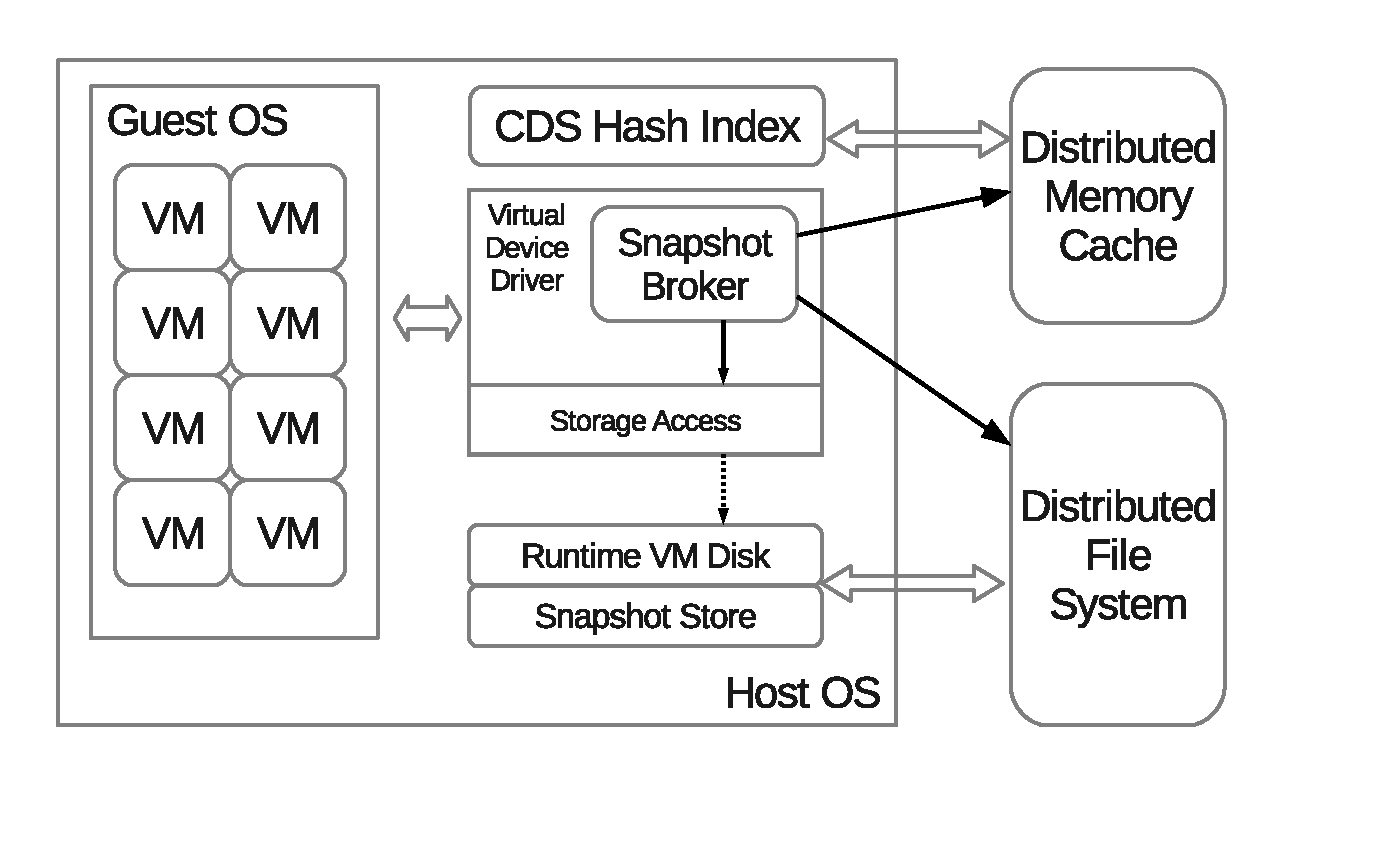
\epsfig{file=images/arch.eps, height=2in, width=2.66in}
  \includegraphics[width=5in]{images/arch1.pdf}
  \caption{Snapshot backup architecture abstraction}
  \label{fig:arch}
\end{figure}

The snapshot store 
supports data access operations such as \emph{Get}, \emph{Append} and \emph{Delete}.
Other operations include data block traverse and resource usage report.
The snapshot data does not need to be
co-located with VM instances, and in fact they can even live in a different cluster to improve the 
data reliability: when one cluster is not available, we are still able to restore its VMs from another cluster which
holds its snapshot data. 
%to reduce the impact to our users.
%Get interface accepts a piece of data, write it to the underline data file, and return
%a reference to the caller. This reference then can be used in the put interface to
%retrive or delete the data, thus the caller of put interface must preserve the
%data reference for future use. 
%In addition to above standand data access operations, the snapshot service also supports
%\emph{scan} and \emph{quota} methods. Scan allows us to traverse all the data blocks of each VM
%in the snapshot store, and quota is used to acknowledge user how much space he
%has actually used.

Under the hood of snapshot store, it organizes and operates snapshot data 
in the distributed file system. We let each virtual disk has its own snapshot store, 
and no data is shared between
any two snapshot stores, thus achieve great fault isolation. For those selected popular data
that shared by many VM snapshot stores, we could easily increase its availability by having more replications.
%Since all the underline data structures is append only,
%upon a delete request, the corresponding data will only be marked rather than being deleted.
%A compaction will take place when deleted data has accumulated to a certain threshold, thus 
%reclaiming the disk space .


%The detail design and implementation of our distributed file system and various 
%storage subsystems would be too complicated to be intorduced here, and also beyond
%the scope of this paper. In the remaining section we will brief the model and interface of 
%our snapshot storage.


\section{Two Level Hierarchical Design of VM Metadata}
\label{overview:meta}

\begin{figure}[htbp]
  \centering
  %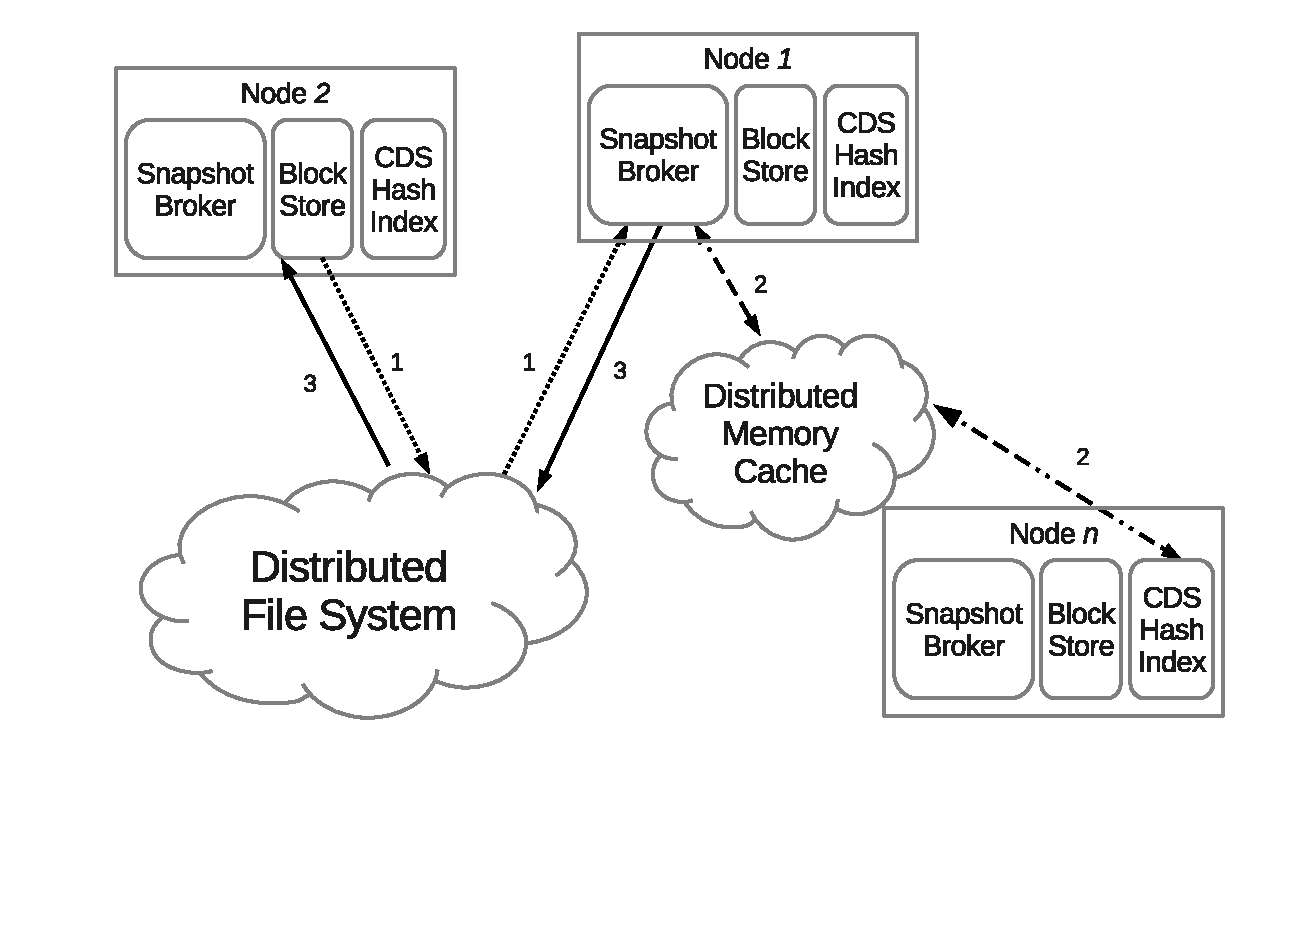
\epsfig{file=images/dedup_process.eps, height=2in, width=2.66in}
  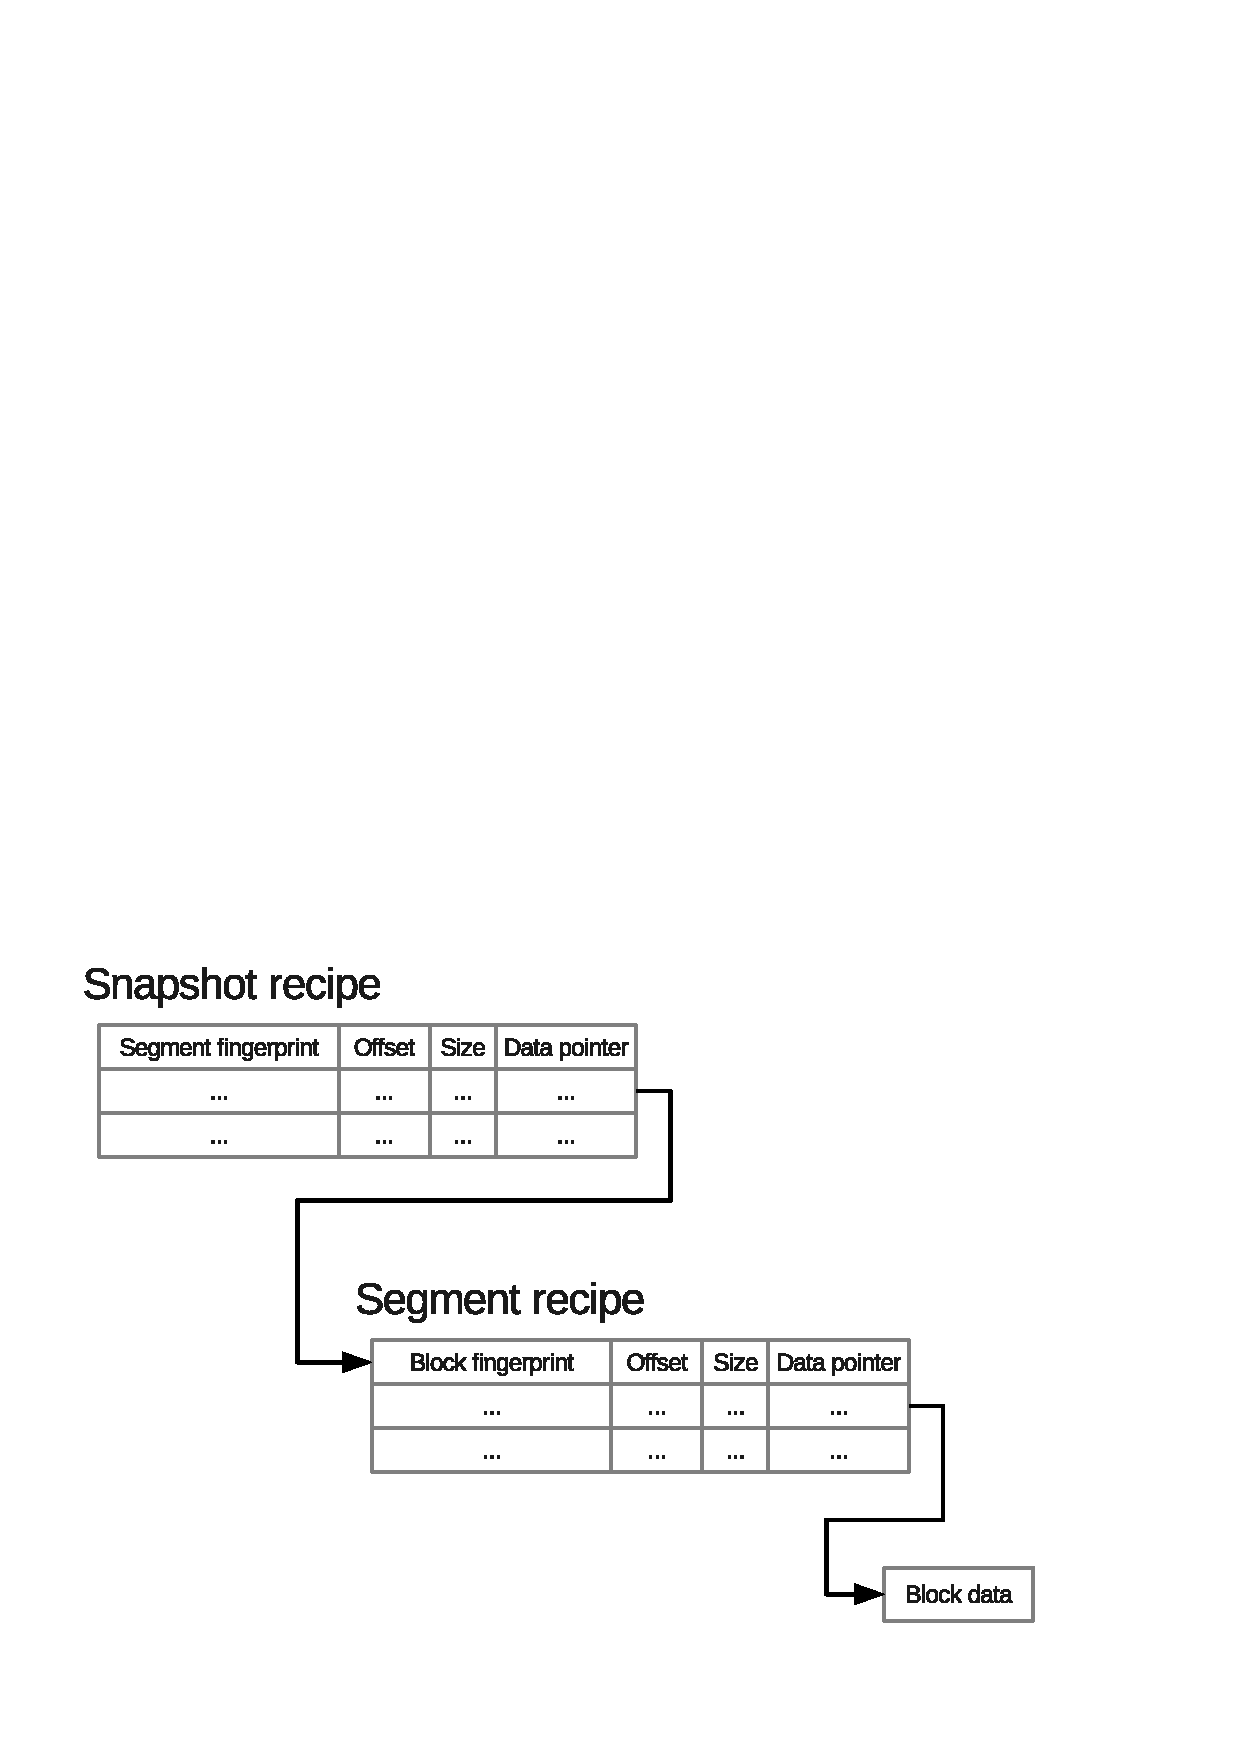
\includegraphics[width=5in]{images/snapshot_representation.pdf}
  \caption{An example of snapshot representation.}
  \label{fig:snapshot}
\end{figure}

The representation of each snapshot in the backup
storage has a two-level index structure in the form of a
hierarchical directed acyclic graph as shown in Figure~\ref{fig:snapshot}.
A VM image is divided into a set of segments and each
segment contains content blocks of variable-size, partitioned using the standard chunking technique with 4KB
as the average block size. The snapshot metadata contains a list of segments and other meta data information.
Segment metadata contains its content block fingerprints
and reference pointers. If a segment is not changed from
one snapshot to another, indicated by a dirty bit embedded in the virtual disk driver, its segment metadata contains a reference pointer to an earlier segment. For a
dirty segment, if one of its blocks is duplicate to another
block in the system, the block metadata contains a reference pointer to the earlier block.


\chapter{Synchronous and Parallel Approach for Offline Deduplication}
\label{chap:offline}
\section{Introduction}
\label{offline:intro}
This chapter introduces a low-cost architecture option and considers that
a backup service uses the existing cloud computing resource.
%Since most of backup data is not used in practice, system resource in such a service is not fully utilized. 
Performing deduplication adds significant  memory cost for comparison of content fingerprints. 
Since each physical machine in a cluster  hosts many VMs, memory contention happens frequently. 
Cloud providers often wish that the backup service only consumes  small or modest resources 
%with a minimal impact to the existing cloud services.  Another challenge for backup with deduplication is 
with a minimal impact to the existing cloud services.  Another challenge is 
%that deletion of old snapshots compete for computing resource as well. That is because data dependence created 
that deletion of old snapshots compete for computing resource as well, because data dependence created 
by duplicate relationship among snapshots  adds processing complexity.

The traditional approach to deduplication is an inline approach which follows
a sequence of block reading, duplicate detection,  and non-duplicate  block write to the 
backup storage. In this chapter we introduce an synchronous and parallel approach
for offline batched deduplication. This solution is suitable for cloud which typically conduct
automatic backup of all the VMs during system's spare time.
Our key idea  is to  first perform parallel duplicate detection for VM content blocks 
among all machines before performing actual data backup. Each machine
accumulates detection requests and  then performs detection   partition by partition 
with minimal resource usage.
Fingerprint based partitioning allows highly parallel duplicate detection  and also simplifies 
reference counting management.  
% as the entire process can also be divided into a
%parition-wise  deletion. 

While our synchronous offline solution accomplishes perfect deduplication efficiency while maintaining
low resource usage,
the tradeoff of this approach is that the job turnaround time for each individual
VM backup task becomes longer. In addition,
every machine has to read dirty segments twice
and that some deduplication requests are delayed for staged parallel processing.
However, with our careful parallelism and buffer management,
this multi-stage detection scheme can provide a sufficient throughput for VM backup.   

The rest of this chapter is organized as follows.
Section~\ref{offline:design} describes our synchronous processing steps.
Section~\ref{offline:eval} is our experimental evaluation that compares with other approaches.
Section~\ref{offline:related} reviews the related works.
Section~\ref{offline:concl} concludes this chapter.

\section{Multi-stage Synchronous Deduplication Design}
\label{offline:design}
We consider deduplication in two levels. The first level
uses coarse-grain segment  dirty bits for version-based detection~\cite{Clements2009,Vrable2009}.
% to identify difference from the previous snapshot to the current snapshot.  
%That  can be accomplished efficiently and inexpensively in the OS level.
%We use a segment-level coarse-grain setting to reduce the efforts in detection and maintaining dirty bits. 
Our experiment with Alibaba's production dataset shows that over 70 percentage of 
duplicates can be detected using segment dirty bits when the segment size is 2M bytes.  
This setting requires OS to maintain segment dirty bits and 
the amount of space for this purpose is negligible. In the second level of deduplication, content blocks of dirty segments 
are compared with the fingerprints of unique  blocks from the previous snapshots.
Our key strategies are explained as follows.
\begin{itemize}


\item {\bf Separation of duplicate detection and data backup.}
%Request accumulation and partition-based deduplication.}
The second level detection requires a global comparison of fingerprints.
% of stored chunks with the new chunks scanned during the backup process. 
%Bloom filters and caching allows some of content 
%fingerprints to be stored on the cheap disks~\cite{bottleneck08}. Such an optimization is good 
%for inline deduplication where chunks scanned need to be determined to be duplicate or not instantly without 
%waiting while  it memory consumption is still significant in competing with stand virtual 
%machine activities.  
Our approach is to perform duplicate detection first before actual data backup.
That requires a prescanning of  dirty VM segments, which
%  and after that, real backup  for those non-duplicates is conducted. 
does incur an extra  round of VM reading.
% while avoiding inline deduplication and leading to a much smaller resource requirement.  
During VM prescanning, detection requests are accumulated.
Aggregated deduplicate requests can be processed partition by partition. 
%We also accumulate the delete requests and perform them partition by partitions. 
Since each partition corresponds to a small portion of global index, 
memory cost to process detection requests within a partition is small.
%the cost to process detection requests within a partition is significantly smaller than processing all 
%the requests globally.

\item {\bf Buffered data redistribution in parallel duplicate detection}.  
Let {\em global index} be the meta data containing the fingerprint values of unique snapshot blocks 
in all VMs and  the reference pointers to the location of raw data.
%A duplicate detection request for a content block needs to be compared with the global index to determine if this
%block is non-duplicate. If it is a duplicate, return the corresponding reference pointer.
%We conduct parallel processing of detection requests in all machines involved. 
A logical way to distribute detection requests among machines is based on 
fingerprint values of content blocks.
% in a  disjointed manner.
Initial data  blocks follows the VM distribution 
among machines 
and the detected duplicate summary 
should be collected following the same distribution.
Therefore, there are two all-to-all data redistribution operations involved.
One is to map detection requests from VM-based distribution to fingerprint based distribution.  
Another one  is to map duplicate summary from fingerprint-based distribution to VM based distribution.  
The redistributed data needs to be accumulated on the disk to reduce the use of memory.
To minimize the disk seek cost, outgoing or incoming data exchange messages are buffered to 
bundle small messages.
Given there are $p\times q$ partitions where $p$ is the number of machines and $q$ is the number of fingerprint-based partitions
at each machine, space per each buffer  is small under the memory constraint for large $p$ or $q$ values.
This counteracts the effort of seek cost reduction.  
%Then there will be a large number of storage  IO operations involved, suffering the huge seek overhead.
We have designed an efficient data exchange and disk data buffering  scheme to address this.

%As we detect and backup requests before actual backup takes place,  we need to store chunk data on 
%temporary disks and once duplicates 
%are detected, we only need to fetch and store these non-duplicates 
%in the backup storage.  To minimize the storage usage of temporary disk space, we donot save the data content 
%of accumulated requests with replication, but we store  data separately for each virtual machine. In an event 
%that the storage of temporary accumulation fails for certain virtual machines, rescanning of these virtual machine images 
%is conducted and backup of these machines is re-initiated.   Meta data such as content hash for accumulated requests 
%is stored separately since we map the meta data into a set of buckets using chunk fingerprints. 
%The benefit of separating content and meta data is to allow fast recovery of backup operations while enabling bucket-based lazy deduplication.

\end{itemize}

We assume a flat architecture in which  all $p$ machines that host VMs in a cluster can 
be used in parallel for deduplication. 
A small amount of local disk space and memory on each machine can be used 
to store global index and temporary data. 
The real backup storage can be either a distributed file system built on
this cluster  or use another  external storage system. 
%Our design is to minimize the usage of local memory and storage on each machine.


%While we assume all machines can process  independent or coordinated
%deduplication and backup operations in parallel,  
%our scheme uses a single-thread procedure on each machine to minimize the use of CPU, network bandwidth, and disk bandwidth.
We use the two level metadata hierachy as discussed in section~\ref{overview:meta}.
The snapshot metadata  contains a list of segments and other meta data information.
Segment metadata contains its  content block fingerprints and reference pointers. 
If a segment is not changed from one snapshot to another, indicated by a dirty bit embedded in the virtual disk driver, 
%its content blocks are not changed as well, thus 
its segment metadata contains a reference pointer to an earlier segment.
For a dirty segment, if one of its blocks is duplicate to another block in the system,  
the block metadata contains a reference pointer to the earlier block.

\begin{sidewaysfigure*}[tbhp]
\centering
\includegraphics[height=0.45\textwidth]{images/steps.pdf}
\caption{Processing flow of Stage  1 (dirty segment scan and request accumulation), Stage 2 
(fingerprint comparison and summary output),  and Stage 3 (non-duplicate block backup).}
\label{fig:flow}
\end{sidewaysfigure*}

%\subsection{Processing flow and resource usage}
The data flow of our multi-stage duplicate detection is depicted in Figure~\ref{fig:flow}. 
%let $v$ be the total number of virtual machines hosted in  a cluster,  
%we divide the backup into $k$  iterations. 
%\begin{itemize}
%\item
In Stage 1, each machine independently reads  
%$v/k$  
VM images that need a backup
and forms duplicate  detection requests. 
%For those dirty segments,
%segments that have been modified since last backup indicated by dirty bits,  
The system divides  each dirty segment into a sequence of chunk blocks,  computes the meta 
information such as chunk fingerprints,  sends a request to a proper machine, and accumulates  
received requests into a partition on the local temporary disk storage. 
The partition mapping uses a hash function applied to the content fingerprint. 
Assuming all machines have a  homogeneous resource configuration, each machine is evenly  assigned with
$q$ partitions of global index and it accumulates corresponding requests on the disk. 
There are two options to allocate buffers at each machine. 
1) Each machine has  $p\times q$ send buffers corresponding to $p\times q$ partitions in the cluster
since a content block in a VM image of this machine can be sent to any of these partitions.
2) Each machine allocates $p$ send buffers to deliver requests to $p$ machines; it allocates 
$p$ receive buffers to collect requests  from other machines.
Then the system copies requests from each of $p$ receive buffers to  $q$ local request buffers,
and outputs each request buffer to one of the request partitions on the disk
when this request buffer becomes full.  Option 2, which is  depicted in Figure~\ref{fig:flow},
is much more efficient than Option 1 because $2p+q$ is much smaller than
$p\times q$, except for the very small  values. 
As a result, each buffer in Option 2 has a bigger size to accumulate requests and that means
less disk seek overhead.

%We assume that the startup cost for network message sending is  much more less (e.g. an order of magnitude
%less) than from one machine to another 
%disk storage startup cost such as seek is much mu
%Note that we only accumulate requests with their meta data information.
%\item
Stage  2 is to load disk data and perform fingerprint comparison at each machine one request partition at a time.
% in the partitions.  
%The system maintains the index of all chunk fingerprints divided in the buckets. 
%The system loads the global index partition 
%and accumulated corresponding requests, and compare them to  identify the duplicated blocks.  
%Then we unload them, load the global index and accumulated requests for another partition. 
%This process is repeated until all buckets are processed.
At each iteration, once in-memory comparison between an index partition and request partition is completed,  
duplicate summary information for segments of each VM is routed from the fingerprint-based distribution  to the
VM-based distribution.  The summary contains the block ID and  the reference pointer for each detected duplicate block.   
Each machine uses memory space of the request partition as a send buffer with no extra memory requirement.
But it needs to allocate $p$ receive buffers to collect duplicate summary from other machines.
It also allocates $v$ request buffers to copy duplicate summary from $p$ receive buffers and output to the local disk
when request buffers are full.

%. In this way, it sends duplicate summary to the corresponding machines one by one to minimize the startup cost for sending a message.
%In the receiving side, 
%All-to-all machines data exchange is conducted  so that  
%each machine allocates $q$ receive buffers corresponding to
%$q$ local partitions, to hold received messages from other machines.  
%When a receive buffer for a VM is  full, the data is written to the local disk storage. 
%These substeps are repeated as the stream of data is exchanged when each machine compares through all $q$ partitions.

%\item 
Stage 3 is to perform real backup.
% one VM at a time.
The system loads the duplicate summary of a VM, 
reads  dirty segments of a VM, and outputs non-duplicate blocks to the final backup 
storage. Additionally, the global index on each machine is updated with the meta data of new chunk blocks. 
When a segment is not dirty, the system only needs to output the segment meta data such as a reference pointer. 
There is an option to directly read dirty blocks instead of fetching a dirty segment which can include duplicate
blocks. Our experiment shows that it is faster to read dirty segments in the tested workload.
Another issue is that during global index update after new block creation,
% in the backup storage,
the system  may find some  blocks with the same fingerprints have been 
created redundantly. For example, two different VM blocks that have the same  fingerprint are not detected
because  the  global index has not contained such a fingerprint yet. 
The redundancy is discovered and logged during the index update and can be repaired
periodically when necessary.  Our experience is that there is a redundancy during the initial snapshot backup and once 
that is repaired, the percentage of redundant blocks due to concurrent processing  is insignificant.

%If a segment is dirty,  the system  use the duplicate summary information from Step 2 for internal 
%duplicate blocks of this dirty segment and output the remaining non-duplicate blocks to the backup storage.
%\end{itemize}

%          In fetching non-duplicates,    it is sometime faster that we fetch a large number of consecutive chunk blocks from an accumulated  segment which contains duplicated chunks,  to avoid the random seek overhead.


The above steps can be executed by each machine using one thread to minimize the use of computing resource.
The  disk storage usage on each machine 
is fairly small for  storing part of global index and
accumulating  duplicate detection requests that contain fingerprint information.   
We impose a memory limit $M$ allocated for each stage of processing at each machine.
The usage of $M$ is controlled as follows and space allocation among buffers is optimized based on the relative
ratio between the cross-machine network  startup cost and disk access startup cost such as seek time.
Using a bigger buffer  can mitigate the impact of slower startup cost. 
\begin{itemize}
\item For Stage 1, $M$  is divided for 
1) an I/O buffer to read dirty segments; 2) $2p$ send/receive buffers and $q$ request  buffers.

%1) $p$ send buffers. images, sends the fingerprint of a dirty block to a machine that is responsible for this fingerprint.
%2) Buffer requests gathered from other machines and divide those requests into $q$ buckets. Once a buffer for each bucket is full, output to the disk storage.
\item 
For Stage 2,  $M$  is divided for 1) space for hosting a global index partition and 
the corresponding request partition; 2) $p$ receive buffers and $v$ summary buffers.
%%accumulating duplicate summary for each targeted VM.   Once  each machine processes a bucket of  duplicate detection requests, 
%For each machine which hosts $v$  VMs, and will receive messages from many other machines, 
%the system needs to allocate buffer space for each VM ot accumulate the duplicate summary records. 
%When a buffer for a VM is full, the result is written to the disk.

\item For Stage 3, $M$  is divided for 1) an I/O buffer to read dirty segments of a VM and   
write non-duplicate blocks to the  backup storage;
2) summary of duplicate blocks within dirty segments. 
\end{itemize}
%We find the memory for step 2 is most critical for buffering duplicate summary in hiding the latency. 
%Certainly most storage system can allow many IO requests issued in parallel overlapping the IO latency.  
%Here we assume the worst case and also minimize the IO bandwidth usages by issuing 
%one request at a time to use the minimal disk bandwidth resource.

{\bf Snapshot deletion.} Each VM will keep a limited number of  automatically-saved snapshots and 
expired snapshots are normally deleted.
% unless its owner explicitly asks for its retention.
We adopt the idea of mark-and-sweep~\cite{Guo2011}. 
A block or a segment can be deleted if its reference count is zero.
%As we discussed in Section~\ref{sect:data}, the reference counter is kept in the global index, partitioned among machines. 
To delete useless  blocks or segments periodically, we read the meta data  of all
snapshots and compute the reference count of all blocks and segments  in parallel.
%while following the fingerprint-based partitioning.
Similar to the multi-stage duplicate detection process, reference counting is conducted in multi-stages. 
Stage  1 is to read  the segment and block  metadata 
to accumulate  reference count requests in different machines  in the fingerprint based distribution.
Stage   2 is to count references within each partition and detect those records with zero 
reference. 
%Stage 3 is that every VM gathers its z confirmed deletion requests for its content and sends them to the backup storage.
The backup  data repository logs deletion instructions,  and will periodically perform a compaction operation when 
its deletion log is too big. 


\section{System Implementation and Experimental Evaluations}
\label{offline:eval}
We have implemented and evaluated a prototype of our multi-stage deduplication scheme on a cluster
of dual quad-core Intel Nehalem 2.4GHz E5530 machines with 24GB memory.  
Our implementation is based on Alibaba's Xen cloud platform~\cite{Aliyun,WeiZhangIEEE}.
Objectives of our evaluation are:
1) Analyze the deduplication throughput and effectiveness for a large number of VMs.
%Compare with the data domain approach~\cite{bottleneck08}.
2) Examine the impacts of buffering during metadata exchange.

%\subsection{Experimental setup}

%We are running our deduplication/backup  service on 100 nodes.
%Memory usage is about 150MB space per node during backup and
%the CPU usage is very small during the experiments. 
We have performed a trace-driven study using  a 1323 VM dataset  collected from 
%100 Alibaba Aliyun's cloud nodes~\cite{WeiZhangIEEE}.
a cloud cluster at Alibaba's Aliyun.
% ~\cite{WeiZhangIEEE}.
% and each of machine nodes has 16 cores and 12 disk drives,  hosting  up to 25 VMs. 
For each VM, the system keeps 10 automatically-backed snapshots in the storage while
a user may instruct extra snapshots to be saved.
The backup of VM snapshots is completed within a few  hours every night.
Based on our study of its production  data,  each VM has about  40GB of storage  data usage on average
including OS and user data disk.
Each VM image is  divided into 2 MB fix-sized segments and each segment is divided into 
variable-sized content blocks  with an average size of 4KB.
%variable sizes~\cite{similar94,rabin81} with an average size of 4KB. 
The signature for variable-sized blocks is computed using their SHA-1 hash. 

The seek cost of each random IO request in our test machines is about  10 milliseconds.
The average I/O usage of local storage is controlled about 50MB/second for backup 
in the presence of other I/O jobs. Noted that a typical 1U server can host
6 to 8  hard drives and deliver over 300MB/second. Our setting uses 16.7\% or less 
of local storage bandwidth. 
The final snapshots are stored in a distributed file system built on the same 
cluster. 

The total local disk usage on each machine is about 8GB for the duplicate detection purpose,
mainly for global index. 
Level 1 segment dirty bits identify 78\% of duplicate blocks. For the remaining dirty segments,
block-wise full deduplication removes about additional 74.5\% of duplicates.
The final content copied to the backup storage is reduced by 94.4\% in total.

\begin{figure}[htbp]
\centering
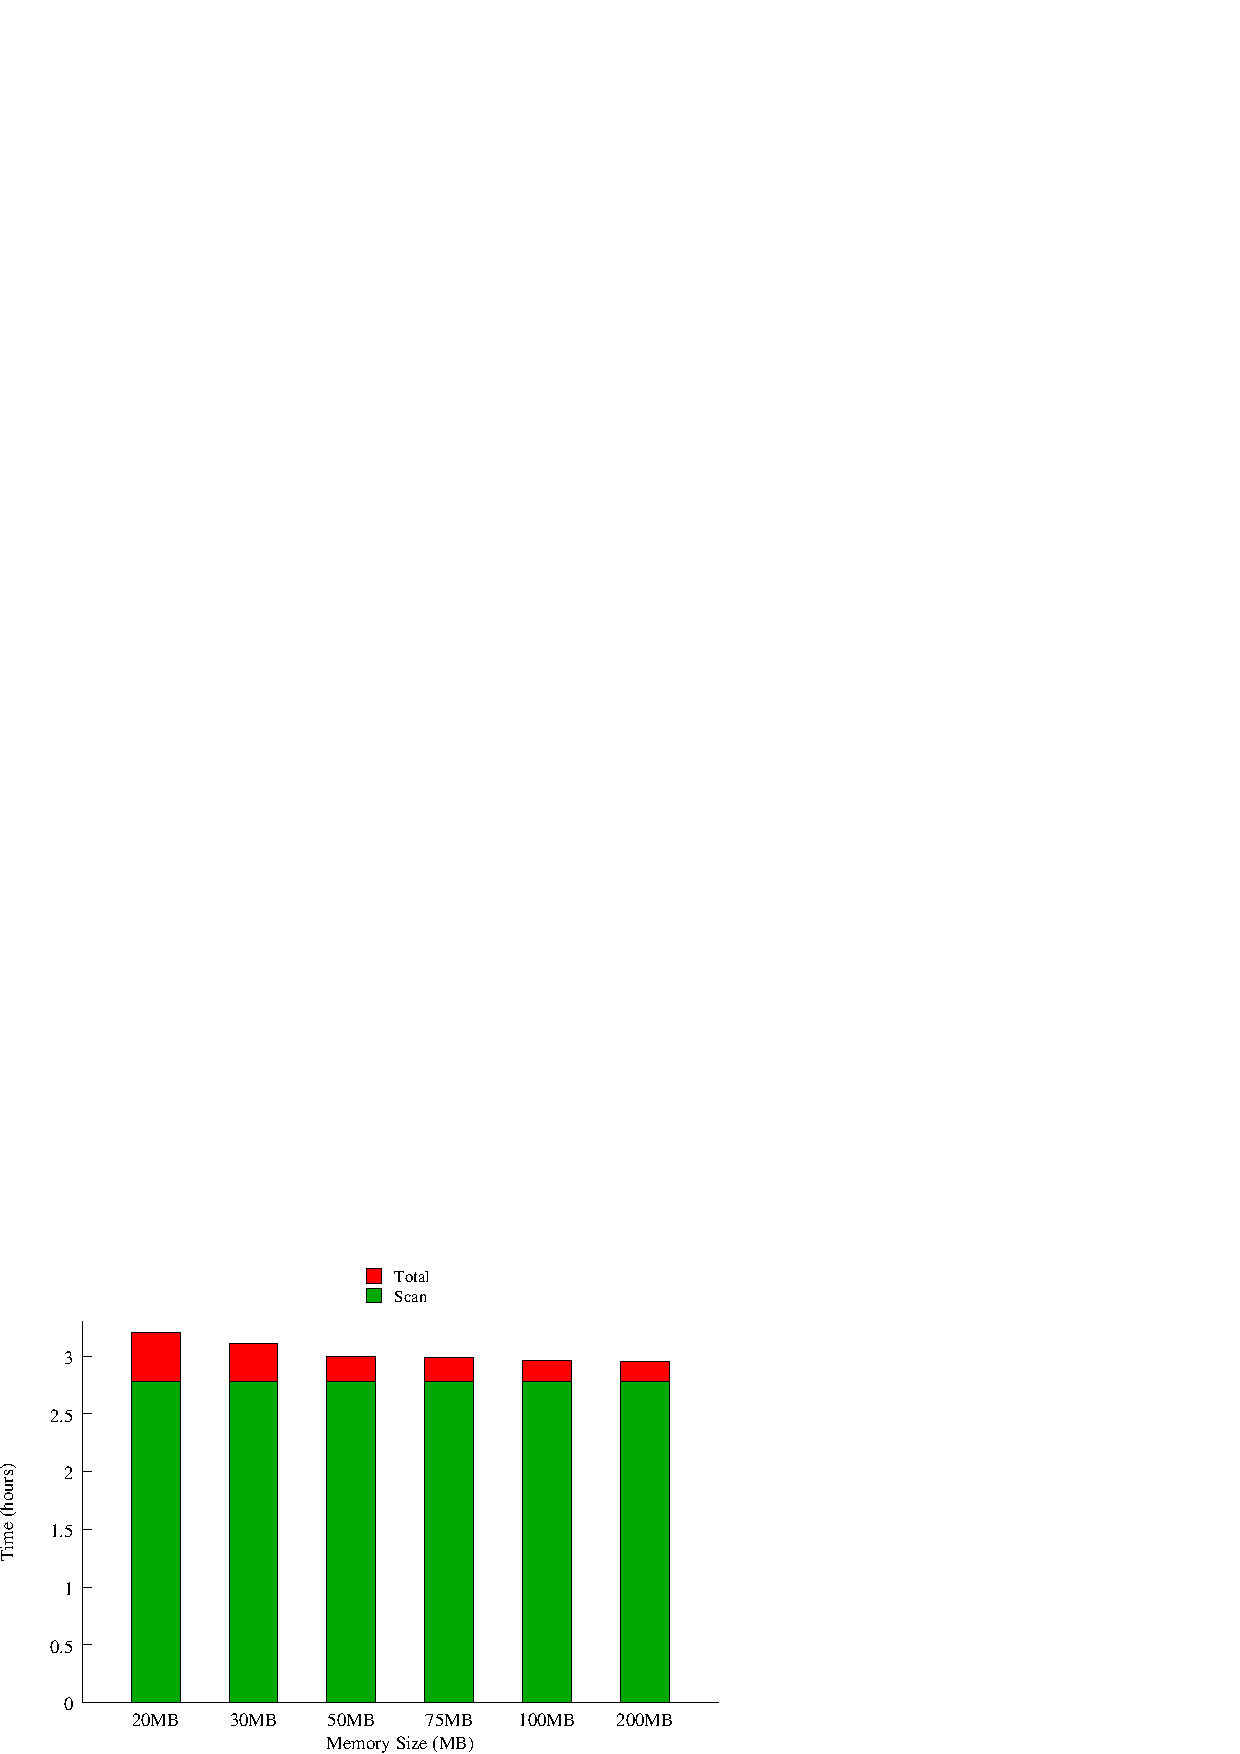
\includegraphics[width=0.6\textwidth]{figures/mem_time.pdf}
\caption{Parallel processing time when memory limit varies.}
\label{fig:memory}
\end{figure}

Figure~\ref{fig:memory} shows the total parallel time in hours to backup 2500 VMs on
 a 100-node cluster a  when 
limit $M$ imposed on each node varies.
%  from 20MB to 200MB.
This figure also depicts the time breakdown for Stages 1, 2, and 3. 
%The parallel time includes the first scanning time, 
%of dirty VM segments to generate block fingerprints, data redistribution for request accumulation,
%fingerprint comparison, duplicate summary distribution, and the second scan time for real backup.
The time in Stages 1 and 3  is  dominated by  the two scans of dirty segments,
and final data copying to the backup storage is overlapped with VM scanning.
During dirty segment reading, the average number of consecutive dirty segments is 2.92. 
%Each scan takes about 1.4 hours.
The overall processing time does not have a significant reduction as $M$ increases to 190MB.
The aggregated deduplication throughput is  about 8.76GB per second,
which is the size of 2500 VM images divided by the parallel time. 
The system runs with  a single thread and  its CPU resource usage is 10-13\% of one core. 
The result shows the backup with multi-stage deduplication  for all VM images can be 
completed in about 3.1 hours with 35MB memory,  8GB disk overhead and a small CPU usage.
As we vary the cluster size $p$,  the parallel time does  not change much, and  the aggregated throughput
scales up linearly since the number of VMs is  $25p$. 

Table~\ref{tab:overall} shows performance change when limit $M$=35MB is imposed and
the number of partitions per machine ($q$) varies.
% varies from 100 to 1000.
Row 2 is memory space required to load a partition of global index and detection requests.
When $q=100$, the required memory is 83.6 MB and this exceeds the limit $M=$35MB.  
Row 3 is the parallel time and Row 4 is  the aggregated throughput of  100 nodes.
%The result shows the backup with multi-phase deduplication  for all VM images can be completed in about 3.09 hours
%with the very small resource usage.
Row 5 is  the parallel time for using Option 1 with $p\times q$ send buffers 
described in Section~\ref{offline:design}. 
When $q$ increases, the available space per buffer reduces and there is a big increase of seek cost.  
The main network usage before performing the final data write is for request accumulation and
summary output. It lasts about 20 minutes and each machine exchanges 
about   8MB of metadata per second with others during that period, which is 6.25\% of the network bandwidth.

\begin{table}[hbt]
\caption{ Performance when $M$=35MB and $q$ varies.}
\begin{center}
\begin{tabular} {|c|c|c|c|c|c|}
\hline \#Partitions ($q$)  & 100 & 250  & 500 &  750 &  1000 \\
\hline Index+request (MB) & 83.6 &  33.5 & 16.8 & 11.2 & 8.45 \\
\hline Total Time (Hours) & N/A&  3.12 & 3.15 & 3.22 & 3.29 \\
\hline Throughput (GB/s) & N/A &  8.76 & 8.67 & 8.48 & 8.30 \\
\hline Total time (Option 1) & N/A&  7.8& 11.7 & 14.8 & 26 \\
\hline
\end{tabular}
\end{center}
\label{tab:overall}
\end{table}


\section{Related Work}
\label{offline:related}
%In a virtualized cloud environment such as ones provided by Amazon EC2\cite{AmazonEC2} and Alibaba Aliyun\cite{Aliyun}, 
At a cloud cluster node, each instance of a guest operating system runs on a virtual machine, accessing virtual hard disks 
represented as virtual disk image files in the host operating system.
For VM snapshot backup, file-level semantics are normally not provided.
Snapshot operations take place at the virtual device driver level, which means no fine-grained file system metadata can be used to determine the changed data. 
%Only raw access information at disk block level are provided. 
%Each physical machine hosts many VMs and petabytes of data in a cloud cluster need a frequent  backup. 
%Ideally speaking, snapshot backup must not affect the normal cloud service, which means that 
%only a very small slice of cluster resource can be used for the backup purpose.

%The previous work for storage backup has extensively used  data deduplication techniques can eliminate redundancy globally among different files from different users.
Backup systems have been developed to use content fingerprints to identify duplicate
content~\cite{venti02,Rhea2008}.
Offline deduplication is 
used in ~\cite{EMC,NetAppOffline} to remove previously written duplicate blocks during idle time.
%,NGmiddleware2011}.
%Today's commercial data backup systems (e.g. from EMC and NetApp)
%\cite{emc_avamar}\cite{datadomain_whitepaper}
%use a variable-size chunking algorithm to detect duplicates in file data~\cite{similar94,hydrastor09}.
Several techniques have been proposed to speedup searching of duplicate
fingerprints. For example, the data domain method ~\cite{bottleneck08} 
uses  an in-memory Bloom filter and a prefetching cache for data blocks  which may be
accessed.  An improvement to this work with parallelization is in ~\cite{MAD210,DEBAR}.
As discussed in Section~\ref{offline:intro},
there is no dedicated resource for deduplication in our targeted setting and low memory usage
 is required so that the resource impact to other cloud services is minimized.
%NG et al.~\cite{ NGmiddleware2011}  use
%a related filtering technique for integrating deduplication in Linux  file system and the memory
%consumed is up to 2GB for a single machine. That is still too big in our context discussed below.
%Lillibridge et al.~\cite{sparseindex09} break list of chunks
%into large segments, the chunk IDs in each incoming segment are sampled and the segment is
%deduplicated by comparing with the chunk IDs of only a few carefully selected backed up segments.
%These are segments that share many chunk IDs with the incoming segment with high probability.
The approximation techniques are studied in~\cite{extreme_binning09,Guo2011}  
%Deepavali et al.~\cite{extreme_binning09} and Zhang et al.~\cite{WeiZhangIEEE}  
to reduce memory requirement with a tradeoff of the reduced deduplication ratio.
%use fingerprint-based file similarity  and group similar files into the same physical location (bins) to deduplicate against each other.
%That leads  to a smaller amount of memory usage for storing meta data in fingerprint
%lookup  
In comparison, this paper focuses on  full deduplication without approximation.
%We also take advantages of the fact that in a VM cloud environment,
%the virtual device driver can easily keep track if  large data
%segments have been modified using dirty bits and such information can avoid sending
%unmodified data segments for deduplication, which significantly saves cost.

Additional inline deduplication techniques are studied in ~\cite{sparseindex09,Guo2011,Srinivasan2012}. 
All of the above approaches have focused on
such inline duplicate detection in which  deduplication of an individual block  is on the critical write path.
In our work, this constraint is relaxed and 
there is a waiting time for many duplicate detection requests. This relaxation is acceptable because 
in our context, finishing the backup of required VM images within a reasonable time window is more
important than optimizing individual VM block  backup requests.

\section{Concluding Remarks}
\label{offline:concl}
The contribution  of this work is a low-cost multi-stage parallel deduplication solution.
Because of separation  of duplicate detection and actual backup,
we are able to evenly distribute  fingerprint comparison among clustered machine
nodes, and only load one partition at time at each machine for in-memory comparison.
%The tradeoff is that every machine has to read dirty segments twice 
%and that some deduplication requests are delayed for staged processing.  

The proposed  scheme is resource-friendly to the existing cloud services.
The evaluation shows that the overall 
deduplication time and throughput of 100 machines  are satisfactory with 
about 8.76GB per second for 2500 VMs. During processing, each machine uses 
35MB memory, 8GB disk space, and 10-13\% of one CPU core with a single thread  execution.
Our future work is to conduct more experiments with production workloads.
%and a modest use of IO and network resource.
%Thus the proposed  scheme does not take a significant  amount of the resource away
%to compete with the existing cloud services.
%While using an insignificant system resource,
%When the cluster size changes, our experiment also shows a linear speedup of overall throughputs
%because highly parallel fingerprint comparisons.  
%The cluster  of 100 nodes and 2500 VMs can deliver about 
%8.8GB per second deduplication performance.  We expect the system performs well in a larger cloud 
%setting and 

The major limitation of our synchronous approach is that all VM snapshots must be processed together
in order to achieve maximum aggregated throughput, as a result, small VMs need to wait big VMs during
the duplicate detection phase until all VMs finishes stage 2. Since the small VM disks 
need to be put under copy-on-write protection longer, their disk I/O performance will be slow down
and  additional disk space are needed to store the modified segments during backup. Another limitation
is that VM user cannot choose the time of taking snapshot freely. Therefore, our synchronous approach 
is ideal for private cloud in which the IT admin needs to backup all the VMs together, but it may not
be suitable 
for public cloud which demands real-time snapshot backup operation. We will discuss our solution
for on demand inline deduplication in the next chapter.


\chapter{Multi-level Selective Approach for Inline Deduplication}
\label{chap:inline}

\section{Introduction}
\label{inline:intro}
In a public virtualized cloud environment such as ones provided by Amazon EC2\cite{AmazonEC2} and Alibaba Aliyun\cite{Aliyun},
VM snapshots are created on user's requests. Because the snapshot captures 
the virtual disk state at a specific point of time,
virtual disk under snapshot backup operation must be protected by copy-on-write until the 
operation finishes. However, copy-on-write introduces additional disk I/O and space overheads, 
users are typically advised to reduce their disk I/O activities to the minimum before making
a snapshot backup operation, such activities typically include their web and database services. 
As a result,
it is critical to perform the backup operation in the shortest amount of time 
to make the VM back to work.

Our synchronous batched deduplication introduced in chapter~\ref{chap:offline} does not apply 
to such situation which requires fast inline deduplication.
Based on the requirement that we are now pursuing low-cost solution with short job turnaround time,
we choose to design a deduplication solution which will sacrifice the deduplication efficiency to 
satisfy the cost and time constraints.
By observations on the VM snapshot data from production cloud, we found snapshot data duplication 
can be easily classified into two categories: \emph{inner-VM} and \emph{cross-VM}. Inner-VM duplication
exists between VM's snapshots, because the majority of data are unchanged during each backup period. 
On the other hand, Cross-VM duplication is mainly due to widely-used software and libraries such as Linux and MySQL.
As the result, different VMs tend to backup large amount of highly similar data.

With these in mind, we have developed a distributed multi-level solution to conduct 
segment-level  and block-level inner-VM  deduplication to localize the deduplication effort when possible.
It then makes cross-VM deduplication by excluding a small number of
popular popular data blocks from being backed up. Our study shows that popular data blocks
occupy significant amount of storage space while they only take
a small amount of resources to deduplicate.
Separating deduplication into multi levels effectively accomplish the major space saving goal
compare the global complete deduplication scheme, at the same time it makes
the backup of different VMs to be independent for better fault tolerance, 
which we will discuss more in chapter~\ref{chap:data}.

%Restricting the scope of global deduplication reduces
%the inter-component  data dependenc during machine failure.

%Several operations are provided for creating and managing snapshots and snapshot trees,
%such as create snapshots, revert to any snapshot, and remove snapshots.
%VM snapshots is different from traditional file system backup from a few aspects:
%\begin{enumerate}
%\item The backup loads are heavy but resources are limited. The whole VM cluster have PBs of data and need to be backuped at daily basis, if not more frequently. But at the same time snapshot tasks must not affect the normal VM operations, which means only a tiny slice of CPU and memory can be used for this purpose.
%\item No file system semantics are provided. Snapshot operations are taken place at the virtual device driver level, which means no fine-grained file system metadata can be used to determine the changed data. Only raw access information at disk block level are provided.
%\item Snapshots can be shared between users. This does not only complicates the parent-child relationship between snapshots, but also require all snapshots be managed in a global namespace.
%\end{enumerate}

%In this paper we intorduce the deduplication scheme of snapshot storage in Aliyun's VM cloud. We exploit the 
The rest of the paper is arranged as follows. 
Section~\ref{inline:options} discusses the requirements and  design options,
Section ~\ref{inline:dedup} presents our multi-level selective deduplication scheme,
Section ~\ref{inline:impl} presents our evaluation results on the effectiveness
of multi-level deduplication for snapshot backup. 
Section ~\ref{inline:related}
discusses on some background and related work.
Section ~\ref{inline:concl} concludes this chapter.

\section{Requirements and Design Options}
\label{inline:options}
We discuss the characteristics and 
main requirements for VM snapshot backup in a cloud environment.
which are different from a traditional data backup. 
% That arises mainly in Alibaba's Aliyun cloud service.
%concerns
%Base on Aliyun's production environment, the snapshot backup job has to satisfy 
\begin{enumerate}
\item {\em Cost consciousness.}
There are tens of thousands of VMs running on a large-scale cluster. 
The amount of data is so huge such that backup cost must be controlled carefully.
On the other hand, the computing resources allocated for snapshot service is very limited
because VM performance has higher priority.  
At Aliyun, it is required that while CPU and disk usage should be small or modest during backup time,
the memory footprint of snapshot service should not exceed 500 MB at each node.

%snapshot service shall not compete cpu, memory, or I/O bandwidth with VMs. Specifically, the memory usage of snapshot service can never exceed 500MB in any node.
\item {\em Fast backup speed.}
Often a cloud has a few hours of light workload each day (e.g. midnight),  which creates an small window for automatic backup.
%But a  longer use of bandwidth and computing resource  for backup can create  noticeable  contention with the existing cloud,
%which is not preferred for cloud production system operation. 
Thus it is desirable that backup for all nodes
can be conducted in parallel and any centralized or  cross-machine communication for
deduplication should not become a bottleneck.
%As a large-scale cluster hosting tens of thousand of active VMs everyday,  the amount of data
%to be processed is huge. 
%For example, in an Aliyun cluster with over 1,000 nodes and each hosts over 25 VMs, The aggreated amount of data 
 % the system must finish saving daily snapshots of all VMs in 2 hours. In our typical 1000 nodes cluster, each node hosts 25 VMs, each VM has 40GB of data on average, that translates to backup throughput of 139GB/second, or 500TB/hour.

% the system must finish saving daily snapshots of all VMs in 2 hours. In our typical 1000 nodes cluster, each node hosts 25 VMs, each VM has 40GB of data on average, that translates to backup throughput of 139GB/second, or 500TB/hour.
\item {\em Fault tolerance.}
The addition of data deduplication should not decrease the degree of
fault tolerance. It's not desirable that small scale of data failure affects the backup of many VMs.
%when users access snapshots in a recovery process. 
\end{enumerate}

There are multiple choices in designing a backup architecture  for VM snapshots.
We discuss the following design options with a consideration on their strengths and weakness.
\begin{enumerate}
\item  {\em An external and dedicated backup storage system.} 
In this architecture setting, a separate backup storage system using
the standard backup and deduplication techniques can be deployed~\cite{bottleneck08,extreme_binning09,sparseindex09}. 
This system is attached to the cloud network and every machine can periodically transfer snapshot data to 
the attached backup system. 
A key weakness of this approach is communication bottleneck between a large number of machines
in a cloud to this centralized  service.
Another weakness is that the cost of allocating separate resource for dedicated backup  can be expensive.
Since most of backup data is not used eventually, CPU and memory resource in such a backup cluster may not be fully utilized.
\item {\em A decentralized and co-hosted backup system with full deduplication.}
In this option, the backup system runs on an existing set of cluster machines.
% and a distributed storage architecture for backup allows a possible exploitation of  data locality between
%the source of data and storage location of backup data. 
The disadvantage is that 
%the backup service would compete CPU, memory, and disk resources with the other cloud services.
even such a  backup service may only use  a fraction of the existing disk storage, 
fingerprint-based search does require a significant amount of memory for fingerprint lookup of searching duplicates.
This competes memory resource  with the existing VMs.
%Decentralized deduplication is studied in ~\cite{Clements2009} and the focus is on
%block-level copy-on-write and compare-by-value techniques.

Even approximation~\cite{extreme_binning09,sparseindex09} can be used to reduce memory requirement,
one key weakness the hasn't been addressed by previous solutions is that global content sharing affects
fault isolation.
Because a content chunk is compared with a content signature collected from other users,
this artificially creates data dependency among different VM users.
% since storage for shared identical content chunks can become a failure point.
In large scale cloud, node failures happen at daily basis,
the loss of a shared block can affect many users whose snapshots share this 
data block. 
Without any control of such data sharing, we can only increase  
replication for global dataset to enhance the availability,
but this incurs significantly more cost.

%we want to isolate 
%each VM's snapshot backup as much as possible while still enjoy the benefit of deduplication.
%In large scale cloud, node faiures happen at daily basis, we don't want a problem at small scale
%to affect large amount of VMs due to data sharing.
%a key weakness of global content fingerprint comparison is that it affects fault isolation.

%2) data sharing among users for accessing popular signagutes causes the system less resilient to storage failures.
%any loss of one piece of  shared data content hash and actualcontent will damange many VM snapshots, which can cause massive impacts
%on reliability of many users.

%Another point is that the previous work in signature-based comparison does not address
%load balancing for a distributed environment during parallel access.  
%Some content signatures can be extremely hot, but the machines  that  handle such signatures can become
% a bottleneck. Uncoordinated signature assignment could lead to imbalanced access workload.
\end{enumerate}


%There are multiple choices of snapshot backup design for VM images and our considerations are described
%as follows. 
%Our design considerations
%\begin{enumerate}
%\item {\bf Centralized vs. decenalized} 
%
%It is desirable to have  a decentralized architecture.
%Given a large amount of snapshot data communicated from each machine to the backup storage,
%with a distributed storage architecture for backup, one could exploit  exploit data locality between
%the source of data and storage location of data to reduce cross-platform bandwidth requirement for backup.

%execute in parallel and easy to coordinate. In fact, we want to avoid cross-node dependency at scheduling VM snapshot operations, such that no global coordinator is necessary.
%\item {Load balancing in resource consumption}: the cost of snapshot service shall be evenly distributed onto every node. We don't have a super powerful
%or stable node that can accept extra responsibility.
%\item {minimization of inter-user data dependency for fault tolerance}: we want to minimize the data dependency to a controllable level. Data deduplication means sharing of data, thus one failure at a single point may affect the snapshot service of hundreds of VMs, which is absolutely unacceptable.
%\item {Resource usage modeling and control}.
%\end{enumerate}

With these considerations in mind, we propose a decentralized backup architecture with multi-level and selective 
deduplication. This service is hosted   in the existing set of machines and resource usage is controlled
with a minimal impact to the existing applications.
The deduplication process is first conducted among snapshots within each VM
and then is conducted across VMs.  
Given the concern that searching duplicates across VMs is a global feature which can affect parallel performance
and complicate failure management,
we only eliminate the duplication of a small but popular data set while still maintaining a cost-effective deduplication ratio.
For this purpose, we exploit the data characteristics of snapshots and collect most popular data.
Data sharing across VMs is limited within this small data set such that adding replicas for it could enhance fault tolerance.

\section{Multi-level Selective Deduplication Scheme}
\label{inline:dedup}
\subsection{Similarity Guided Inner-VM Deduplication}
\label{sect:innerVM}
The first-level deduplication is logically localized within each VM.
%There are several reasons that we let each MS have  its own block store for localized duplication rather than sharing. 
%First, all data written to block store are already being processed by deduplication
%process, thus no sharing is necessary unless we want to perform additional deduplication
%inside the block store. Second, 
Such localization increases data independency between different  VM backups,
simplifies  snapshot  management and statistics collection during VM migration and termination,
and facilitates parallel execution of snapshot operations.
%Finally, this reduces the complexity of concurrent snapshot operations.

%\begin{figure}[htbp]
%  \centering
%  %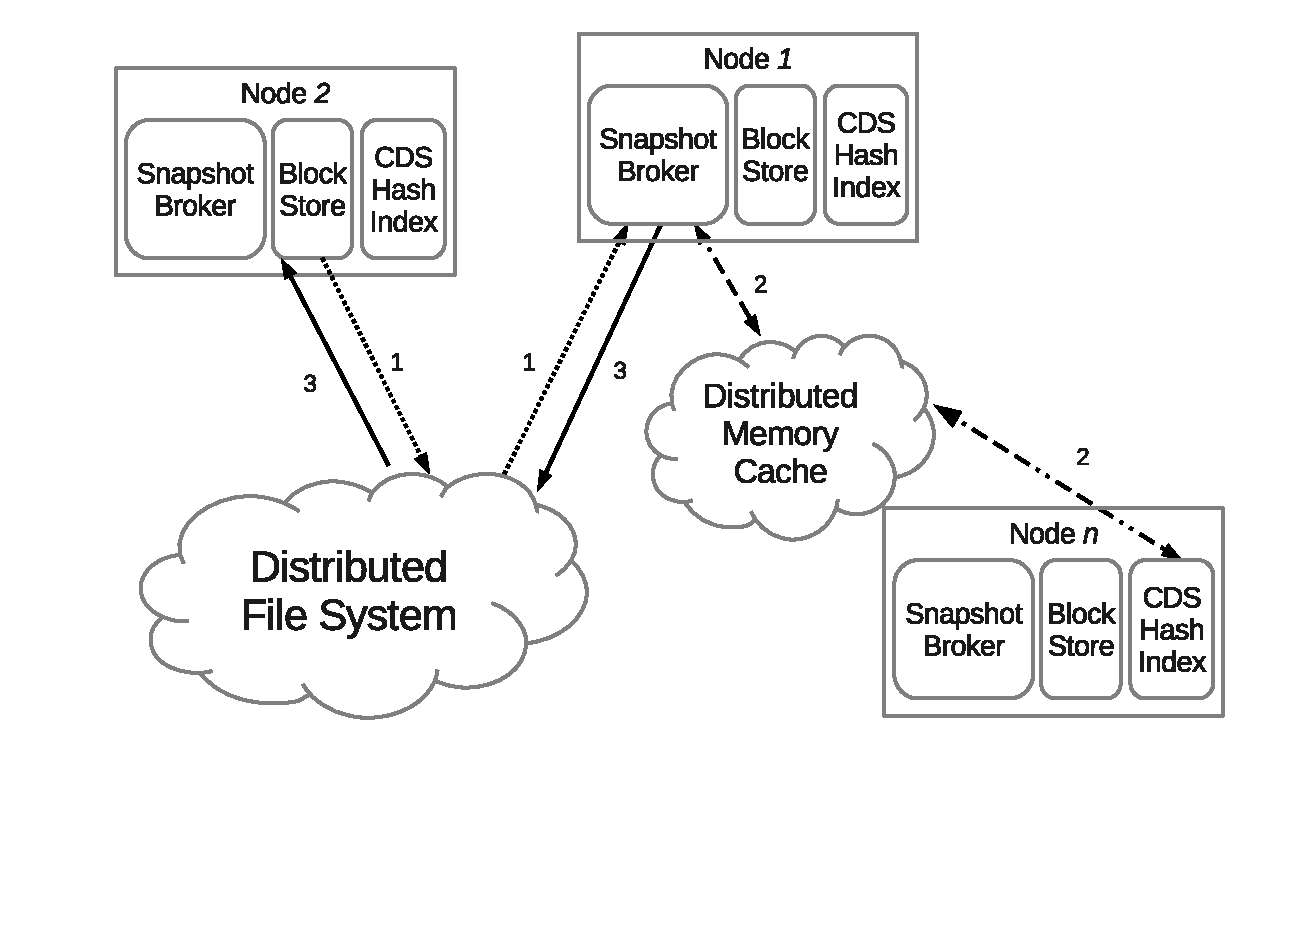
\epsfig{file=images/dedup_process.eps, height=2in, width=2.66in}
%  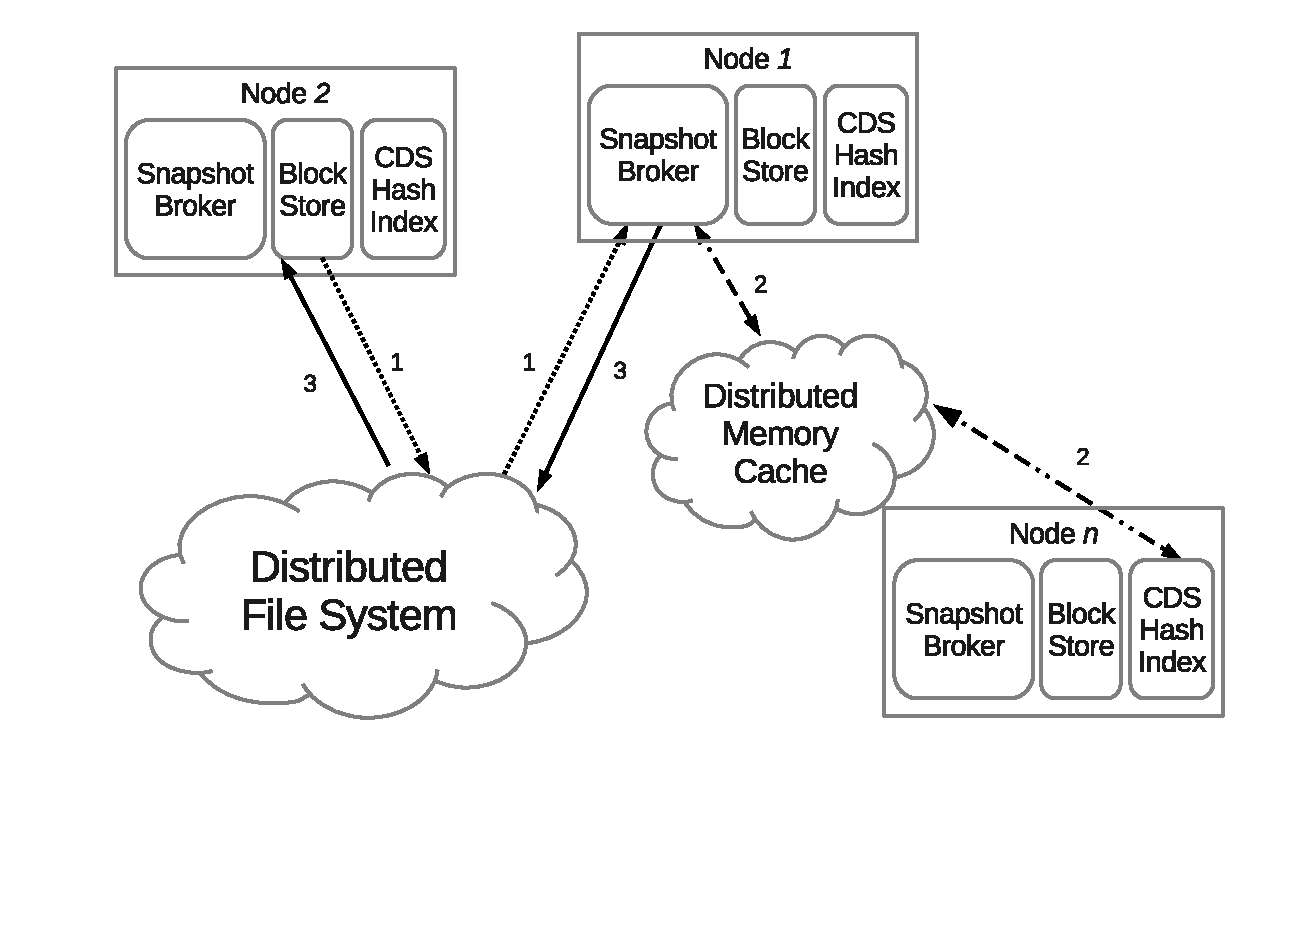
\epsfig{file=images/dedup_process.eps,  width=3.2in}
%  \caption{An example  of multi-level deduplication process.}
%  \label{fig:arch}
%\end{figure}

The inner VM deduplication contains two levels of duplicate detection efforts and the representation of
each snapshot is correspondingly designed as a two-level level index data structure in the form of a hierarchical
directed acyclic graph as shown in Figure~\ref{fig:snapshot}.
An image file is divided into a set of segments and each  segment contains hundreds of content blocks from the bottom level.
These blocks are of variable-size, partitioned using
the standard chunking technique~\cite{similar94} with 4KB as the average block size. 
%To simplify the deduplication process, segments are aligned to fix-sized boundaries, currently using 2MB.
Segment metadata (called segment recipe) records its  content block hashes and data pointers. 
The snapshot recipe contains a list of segments and other meta data information.
\begin{itemize}
\item {\em Level 1 Changed segment tracking}.
% If a segment is not changed, indicated by a dirty bit embedded in the virtual disk driver, its content blocks are not changed as well, thus its segment recipe can be simply reused. Operations at this level have almost no cost and most of unmodified data are filtered here. 
We start with the changed block tracking approach in a coarse grain segment level.
In our implementation with Xen on an Alibaba platform, the segment size is 2 MB
and the device driver is extended to support tracking changed segments using a dirty bitmap. 
Since every write for a segment will touch a dirty bit, the device driver maintains dirty bits in memory
and cannot afford a small segment size.
It should be noted that dirty bit tracking is supported or can be easily implemented in 
major virtualization solution vendors. For example,
the VMWare hypervisor has an API to let external backup applications know 
the changed areas since last backup. 
The Microsoft SDK provides an API that allows external applications to monitor 
the VM's I/O traffic and implement such changed block tracking feature.

\item {\em Level 2  Similarity guided segment comparison.}
% If a segment is modified, we perform fine-grained deduplication using content blocks of this segment to compared with 
% the same segment in
% the previous snapshot (also called parent snapshot). Partial duplication
% within the segment can be detected and eliminated. 
Since the best deduplication uses a non-uniform chunk size 
in the average of 4KB or 8KB~\cite{Jin2009},
we conduct additional local similarity guided deduplication on a snapshot by comparing
chunk fingerprints of a dirty segment 
with those in  {\em similar} segments from its parent snapshot. 
We define two segments are similar if their content signature is the same.
This segment content signature value is defined as the minimum value of all its chunk fingerprints 
computed during backup and is recorded in the snapshot metadata (called recipe). Note that this definition of
content similarity is an approximation~\cite{resemblance97}.  When processing a dirty segment,
its  similar segments can be found easily from the
parent snapshot recipe.  Then recipes of the similar segments are loaded to memory,
which contain chunk fingerprints to be compared.
To control the time cost of search, we set a limit on the number of  similar segments recipes to be fetched. 
For a 2MB segment, its segment recipe is roughly 19KB which contains about 500 chunk fingerprints and other chunk metadata,
by limiting at most 10 similar segments to search, the amount of memory for maintaining those similar segment recipes is small.
As part of our local duplicate search we also compare the current segment
against the parent segment at the same offset.

\end{itemize}

We choose this two-level structure because in practice we observe that during each backup period only a small amount
of VM data are added or modified. As the result, even the metadata of two snapshots can be highly similar,
thus aggregating a large number of content blocks as one segment can significantly
reduce the space cost of snapshot meta data. 
%Namely the  snapshort metadata starts with
%the representation of segment-level meta data. Each segment receipe can be further represented by
%a set of content block receipes.

How can we choose the length of a segment?
Instead of using variables-sized segments, we take a simple approach
to let every segment being aligned to the page boundary of each virtual image file.
For Aliyun, each VM image file is represented as a virtual disk file format
(called \emph{vhd} at Xen) and we use a dirty bit to capture if a page (or segment) of a virtual disk file 
has been modified or not to ease the segment-level deduplication.
%This is effective because  
%a vhd   file keeps the allocated inner blocks at the same positions until deletion,
%which means the locality of snapshot data is almost natively aligned. 
A dirty bit array is used to indicate which segments have been modified or not. 
Each page (segment) size in our implementation uses 2 MB, which contains a large number of content blocks.
%Enforcing a boundary at every 2MB will 
%only break 0.2\% of total data blocks which is tiny.
% dirty bits array. This is because
%Inside the TapDisk driver, we maintain an array of \emph{dirty bits} to record the dirty area
%of runtime VM image file since the last snapshot, each bit represent a 2MB fix-sized
%data segment. During a snapshot operation, we only need to look at the dirty region
%rather than scan over the whold image file, which would be extremely slow.


%We let each virtual disk has its own block store rather than sharing for several reasons:
%first, all data written to block store are already being processed by deduplication
%process, thus no sharing is necessary unless we want to perform additional deduplication
%inside the block store. Second, such seperation will facilitate VM data stastics, 
%deletion and migration. Finally, this reduces the complexity of concurrent snapshot operations.

Once level-2 deduplication is activated for those segments that have been modified,
it requires memory to load  block fingerprints from the corresponding
parent snapshot's segment.
This scheme processes one segment at time and each segment of 2 MB contains about 
500 content blocks on average given 4KB is the average block size.
That only takes a tiny amount of space to hold their fingerprints.
%Given  1-2 hours of window to backup snapshots and every VM has  on average about 40GB, there is enough
%time to search all segments sequentially~\cite{NOT-CLEAR-HERE}

\subsection{Popularity guided Cross-VM Deduplication with PDS}
\label{sect:crossVM}

The level-3 deduplication is to identify duplicated data blocks among multiple VMs through the index cache
of popular data set (PDS).  PDS is the most popular content blocks 
among snapshots across all VMs. 
Each index entry contains  the block fingerprint and a reference pointer to the location of its real content
in the snapshot content block store.
%The structure of PDS meta is not different from the segment recipe we discussed above, 
%except that it is partitioned into many small slices so that each node is easy to load its own slice. 

At the runtime, the PDS index resides in a distributed  memory lookup table  
implemented using Memcached~\cite{memcached} to leverage the aggregated memory in a cluster.
The usage of memory at each machine is small and thus  this scheme  does not
lead to  a memory resource contention with the existing cloud services.
PDS raw data stored  in the distributed file system
has multiple copies in different machines for the purpose of fault tolerance and 
while providing high read throughput.  

To control the size of searchable popular data in this global setting, we focus on those items that 
are most popular based on the historical snapshot data and the popular analysis is conducted periodically to ensure 
meta data freshness to match the latest data access trend.
There are two advantages to exploit this.
First, a smaller PDS reduces overall resource requirement while covering most of data duplication.
Second, knowing this small set of data is shared heavily makes the fault tolerance management 
easier because we can replicate more copies to mitigate the failure.

\begin{figure}[htbp]
\centering
\includegraphics[width=5in]{images/vector.pdf}
\caption{Number of duplicates vesus ranking}
\label{fig:zipf-data}
\end{figure}

In Aliyun's VM cloud, each VM explicitly maintains  one OS disk, plus one or more data disks.
During VM's creation, its OS disk is directly copied from user's chosen base image.
Given the separation of OS disks and data disks, we study  their characteristics separately.
We expect that data related to OS and popular software installations are not frequently
modified or deleted, to facilitate analysis we call them \emph{OS-related} data, 
and the rest of data, either from OS or data disks, are called \emph{user-related} data.
%base image data as a hint.Through users may change configurations, install software, or write user data into OS disk,
%Thus most of content blocks for the OS related snapshots  shall keep unchanged.
%This is verified in  Section~\ref{sect:exper}.

We have studied the popularity of popular blocks in the OS and data disks from a dataset
containing over 1,000 VMs, taking their first snapshots to watch the cross-VM duplication pattern 
(scale of OS disk sampling is smaller due to performance impact to user VMs).
Figure \ref{fig:zipf-data} shows the duplicate count for unique data blocks sorted by their ranking in 
terms of the duplication count. $Y$ axis is the popularity of a data block in a log scale 
measured its duplicate count among snapshots. $X$ axis is the identification of data blocks in a log scale
sorted by their duplicate rank.  The rank number 1 is the block with the highest number of duplicates.
These two curves exhibit that the popularity of popular blocks partially follows a Zipf-like distribution.
%$Y$ axis is the popularity of an OS block in a log scale 
%measured its duplicate count among snapshots. $X$ axis is the identification of OS blocks in a log scale
%sorted by their duplicate rank.  
%For the top ranked blocks, there is a flat line in terms of duplicate counts. That
%is because there are a large number of OS blocks which have appeared in all copies of such OS releases.




%\epsfig{file=images/log-log.disk.eps, width=3in}

%\begin{tabular}{cc}
%\epsfig{file=images/datadisk.count_rank.eps, width=1.5in} &
%\epsfig{file=images/35vmos.count-rank.eps,width=1.5in}
%\end{tabular}


%\begin{figure}
%\centering
%\epsfig{file=images/35vmos.count-rank.eps,width=3in}
%\caption{ Duplicate count of  popular OS blocks in a log scale.}
%\label{fig:OSpopular}
%\end{figure}

Base on the Zipf-like distribution pattern, many previous analysis and results on web caching\cite{Adamic2002,Breslau1999b} may apply.
In general this indicates a small set of popular data dominates data duplication.
Although we already know OS-related data are heavily duplicated among OS disks, 
it still surprises us that user-related data follow a similar pattern.
Therefore, we collect the PDS by performing global reference counting through map-reduce for all
blocks in snapshot store, and select the most popular ones base on the memory limitation of
PDS hash index. 

The PDS collected from user-related data is generally proportional to the data size.
As discussed in Section~\ref{inline:impl}, selecting about 1\% of data (after level 1 and level 2 deduplication)
can cover about 38\% of data blocks. Consider we allow maximum 25 VMs per machine, each VM has
about 30 GB of user-related data, having 10 snapshots in its snapshot store and the data change ratio during
each backup is 10\%, this translates to 15 GB PDS data per machine. 
Consider each PDS hash index entry cost about 40 bytes and the average block size is 4KB, this leads to
a 1:100 ratio so the 
memory cost by PDS hash index is about 150 MB per machine.
On the other hand, the PDS from OS-related data is only relevant to the number of OS releases.
Our experiment on 7 major OS releases shows that about 100 GB of data is never modified, and we expect
it won't grow over 200 GB in the near future. So it would cost the entire cluster 2 GB of memory to
store its hash index, or 20 MB per machine on a 100 node cluster. On average each OS disk has about 10 GB
of data that can be completely eliminated in this way.
Thus in total the PDS index size per node takes less than 170 MB in a large cluster bigger than 100 nodes, 
covering over 47\% of blocks in OS and data disks after inner-VM deduplication.
This memory usage is well below the limit required by our VM services.

\subsection{Illustration of multi-level deduplication process}

%%Our deduplication process is divided into three levels, at each level, we eliminate the most of duplicate data with available knowledge, preventing them from going further because deduplication at deeper level is more expensive.
%
\begin{figure}
  \centering
  \includegraphics[width=5in]{images/dedup_flow2.pdf}
  \caption{Illustration of snapshot deduplication dataflow.}
  \label{fig:dedupflow}
\end{figure}

We illustrate the steps of 3-level deduplication in Figure~\ref{fig:dedupflow}, which can be summarized as 5 steps:
\begin{enumerate}
\item {\em Segment level checkup.}
As shown in Figure~\ref{fig:dedupflow} (a),
when  a snapshot of a plain virtual disk file is being created, we first check the dirty bitmap 
to see which segments are modified. If a segment is not modified since last snapshot, 
it's data pointer in the recipe of the  parent snapshot  can be directly copied into 
current snapshot recipe (shown as the shadow area in Figure~\ref{fig:dedupflow} (b)).

\item {\em Block level checkup.}
As shown in Figure~\ref{fig:dedupflow} (b),
for each dirty segment, we divide it into variable-sized blocks,
and compare their signatures with  the similar segment recipes in the previous snapshot (called parent
snapshot). 
For any duplicated block, we copy the data pointer directly from the parent segment recipe. 
\item {\em PDS checkup.} For the remaining  content blocks whose duplicate status is unknown,
Figure~\ref{fig:dedupflow} (d)
shows  a further check to compare  them with  the cached signatures in the PDS by querying
the PDS hash index. If there is a match, the corresponding data pointer from the PDS index is
copied into the segment recipe. 
\item {\em Write new snapshot blocks :}
If a data block cannot be found in the PDS index, this block is considered to be a new block
and such a block is to be saved in the snapshot store, the returned data pointer is
saved in the  segment recipe.
\item {\em Save recipes.} Finally the  segment recipes are saved in the  snapshot block store also.
 After all segment recipes are saved, the snapshot recipe is complete and can be saved.
\end{enumerate}

If there is no parent snapshot available, which happens when a VM creates its first snapshot, 
only PDS-based checkup will be conducted. 
Most of the cross-VM duplication, such as OS-related data, is eliminated
at this stage. 


\section{System Implementation and Experimental Evaluations}
\label{inline:impl}
We have implemented the snapshot deduplication scheme on the Aliyun's cloud platform.
Objectives of our experimental evaluation are:
1) Analyze the popularity of content data blocks and the popularity  of hot items.
2) Assess the effectiveness  of 3-level deduplication for reducing the storage cost of snapshot
backup.
3) Examine the impacts of PDS size on deduplication ratio.

\subsection{Experimental setup}

At Aliyun our target is to backup cluster up to 1000 nodes
with 25 VMs on each.
%We are running our deduplication/backup  service on 100 nodes.
%Memory usage is about 150MB space per node during backup and
%the CPU usage is very small during the experiments.
Based on the data studied,  each VM has about  40 GB of storage  data usage on average,
OS disk and data disk each takes about 50\% of storage space.
The backup of VM snapshots is completed within two hours every day,
and that translates to a backup throughput of 139 GB per second, or 500TB per hour.
For each VM, the system keeps 10 automatically-backed snapshots in the storage while
a user may instruct extra snapshots to be saved.

% the system must finish saving daily snapshots of all VMs in 2 hours. In our typical 1000 nodes cluster, each node hosts 25 VMs, each VM has 40GB of data on average, that translates to backup throughput of 139GB/second, or 500TB/hour.

%In our snapshot deduplication architecture, PDS is the key to achieve greater deduplication than
%incremental backup solutions. Our basic assumption of PDS us that VM disks, especially OS disks,
%have huge amount of data in popular, and such popular data can be represented by a relatively smaller data set
%because of their high appearence frequency. As a result, the major portion of snapshot deduplication effect shall
%emerge from eliminating the duplication of such a small data set. In this section, we evaluate
%the effectiveness of PDS using real user VM disks from our production VM cluster.

Since it's impossible to perform large scale analysis without affecting the VM performance,
we sampled two data sets from real user VMs to measure the effectiveness of our deduplication scheme.
Dataset1 is used study the detail impact of 3-level deduplication process,
it compose of 35 VMs from 7 popular OSes:
Debian, Ubuntu, Redhat, CentOS, Win2003 32bit, Win2003 64 bit and Win2008 64 bit. For each OS,
5 VMs are chosen, and every VM come with 10 full snapshots of it OS and data disk.
The overall data size for this 700 full snapshots is 17.6 TB.

Dataset2 contains the first snapshots of 1323 VMs' data disks from a small cluster with 100 nodes.
Since inner-VM deduplication is not involved in the first snapshot, this data set helps us to
study the PDS deduplication against user-related data. The overall size of dataset2 is 23.5 TB.

All data are divided into 2 MB fix-sized segments and each segment is divided into
variable-sized content blocks ~\cite{similar94,rabin81} with an average size of 4KB.
The signature for variable-sized blocks is computed using their SHA-1 hash.
Popularity of data blocks are collected through global counting
and the top 1\% will fall into PDS, as discussed in Section~\ref{sect:crossVM}.


%To compare the effectiveness with a full deduplication approach with an approximation,
%we use  extreme binning and perfect deduplication~\cite{extreme_binning09}.
%For perfect deduplication and extreme binning, each snapshot is also divided into chunk blocks
%using TTTD with an average size of 4KB. The original extreme binning work uses the whole file
%as the input unit and  this size is too big in our system.
%Thus we split each image snapshot file into variable-sized segments base on the block hash list,
%using TTTD with average size of 2MB.

\subsection{Effectiveness of Multi-level Deduplication}

\begin{figure}
  \centering
  \includegraphics[width=5in]{images/overall_effect.pdf}
  \caption{Impacts of 3-level deduplication. The height of each bar is the data size after
deduplication divided by the original data size and the unit is percentage. }
  \label{fig:overall}
\end{figure}

Figure~\ref{fig:overall} shows the overall impact of 3-level deduplication on dataset1.
The X axis shows the overall impact in (a),  impact on OS disks in (b), and impact on data disks in (c).
Each bar in the Y axis shows the data size after deduplication divided by the original data size.
Level-1 elimination can reduce the data size to about 23\% of original data, namely it delivers close 77\% reduction.
Level-2 elimination is applied to data that could pass level-1, it
reduces the size further to about 18.5\% of original size, namely it delivers additional 4.5\% reduction.
Level-3 elimination together with level 1 and 2
reduces the size further to 8\% of original size, namely it delivers additional 10.5\% reduction.
Level 2 elimination is more visible in OS disk than data disk, because data change frequency is really small
when we sample last 10 snapshots of each user in 10 days. Nevertheless, the overall impact of level 2 is still significant.
A 4.5\% of reduction from the original data represents about 450TB space saving for a 1000-node cluster.


\begin{figure}
  \centering
 %\epsfig{file=images/os_cds_sim.eps, width=3in}
  \includegraphics[width=5in]{images/3level_os.pdf}
  \caption{Impact of 3-level deduplication for OS releases.}
  \label{fig:oscds}
\end{figure}

%To see the impact of multi-level deduplication on different OS releases,
%Some of  OS disks are modified frequently and in some cases,  users even store a large amount of user data on
Figure~\ref{fig:oscds} shows the impact of different levels of deduplication for different OS releases.
In this experiment, we tag each block in 350 OS disk snapshots from dataset1 as  ``new''
if this block cannot be deduplicated by our scheme and thus has to be written to the snapshot store;
``PDS''  if this block can be found  in PDS;
``Parent segment'' if  this block is marked unchanged in parent's segment recipe.
``Parent block'' if  this block is marked unchanged in parent's block recipe.
With this tagging, we compute the percentage of deduplication accomplished by each level.
As we can see from Figure~\ref{fig:oscds}, level-1 deduplication accomplishes a large percentage of elimination,
this is because the time interval between two snapshots in our dataset
is quite short and the Aliyun cloud service makes a snapshot  everyday  for each VM.
On the other hand,  PDS still finds lots of duplicates that inner VM deduplication can't find,
contributing about 10\% of reduction on average.

It is noticeable that level-1 deduplication doesn't work well for CentOS, a significant percentage of data is not
eliminated until they reach level-3. It shows that even user upgrade his VM system heavily and frequently
such that data locality is totally lost, those OS-related data can still be identified at level-3.

In general we see a stable data reduction ratio for all OS varieties, ranging from 92\% to 97\%, that means
the storage cost of 10 full snapshots combined is still smaller than the original disk size. And compare to
today's widely used copy-on-write snapshot technique, which is similar to our level-1 deduplication, our
solution cut the snapshot storage cost by 64\%.


%Combining OS disks in all the VMs, we see the overall 7.4TB of data is reduced to 512GB.
%The extreme binning approach can reduce this data set to 542GB, which is slightly worse. As a reference,
%perfect deduplication achieves 364GB in this experiment.

%Overall speaking, inner   VM deduplication or  PDS-based deduplication
%can work well alone, but by combining them together we get a fairly good and stable deduplication ratio to
%all kind of OSes.
%Compared to a traditional dirty bit approach based on pages of
%each file (e.g. segment in our scheme),
%our PDS-based level 3 approach  can save additional 50\% storage space because many of level 2 block
%content can be eliminated using the PDS also.

\subsection{Coverage of popular data blocks}

%We study characteristics of popular data blocks among snapshots of VM users
%and examine the impacts if we only store a relative small amount of popular data blocks to be sored in the PDS server.
%There are two advantages to exploit this.
%First, a smaller PDS reduces overall resource requirement while covering  most of data blocks in snapshots.
%Second a smaller PDS makes the fault tolerance management  easier because we can replicate  more copies
%to mitigate the failure.

%We consider each virtual disk contains two parts: OS partition and regular user data partition
%and study their characteristics seperately.
%In Aliyun's VM cloud, each VM explicitly maintains  one OS disk, plus  one or more data disks.
%During VM's creation, its OS disk is directly copied from user's choosen base image.
%Since  they dare brought by the operating system and popular
%software installations,  they are rarely modified or deleted.
%base image data as a hint.
%Through users may change configurations, install software, or write user data into OS disk,
%but most of the OS related data shall keep unchanged.

%Previous study has also supported this\cite{vmimage}. Therefore, we can let all OS disks share these
%popular data in their snapshot backups.
%We choose user's data disks rather than OS disks in thie experiment for several reasons: First, the data in OS disks are
%instinctively highly similar, because most of the VM users only make some popular or unique but tiny changes to their OSes,
%so the data duplication pattern in OS disks cannot reflect the real distribution of general user data.
%Second, the data disks are way more important in terms of data safty and backup because they are
%what users really care about.

%Furthermore, our study on user's data disks has shown that the duplication pattern of
%variable-sized data blocks follows \emph{Zipf-like} distribution. As a result, the major portion of
%deduplication effect will emerge from eliminating the duplication of frequently seen data.
%define PDS

\begin{figure}
\centering
\includegraphics[width=5in]{images/ay41a_big_data_disk_cdf.pdf}
\caption{Cumulative  coverage of popular popular user data blocks.}
\label{fig:userdatacoverage}
\end{figure}

One of our biggest advantage is small memory footprint for deduplication, because we only
eliminate a small amount of highly popular data.
we use dataset2 to demonstrate the coverage of popular data blocks on user-related data,
as shown in Figure \ref{fig:userdatacoverage}.
%content blocks used in image files using 90\% of
%the collected dataset.
%Figure \ref{fig:userdatacoverage} shows the cumulative coverage  ratio of  popular popular user data blocks.
The $X$ axis is the rank of popular user data blocks, and $Y$ shows how much raw data can be covered given
the size of PDS.
Let $S_i$ and $F_I$ be the size and duplicate count
of the $i$-th block ranked by its duplicate rank.  Then $Y$ axis is the coverage of
the popular dataset covering data items from rank 1 to rank $i$. Namely
\[
\frac{ \sum_{i=1}^{i} S_i * F_i} {\mbox{Total data size}}.
\]

Thus with about 1\% of blocks on data disks, PDS can cover about 38\% of total data blocks
appeared in all data snapshots. The corresponding PDS index uses no more than 150 MB memory per machine,
which can be easily co-located with other cloud services.

%Figure~\ref{fig:OSdatacoverage} shows the cumulative coverage  ratio of  popular popular OS blocks.
%From both graphs, a small number of most popular popular blocks can coverage a large percentage of
%snapshot blocks and thus the size of PDS can be chosen to be small while still having a large
%coverage.

%\begin{figure}
%\centering
%\epsfig{file=images/ay41a_small.os_incremental.cdf.eps, width=3in}
%\caption{ Cumulative  coverage of popular popular OS disk blocks.}
%\label{fig:OSdatacoverage}
%\end{figure}


%We define \emph{OS PDS} to be the unchanged data across the base VM image and the snapshots of all
%OS disks which are derived from it. Such data are brought by the operating system and popular
%software installations, they are rarely modified or deleted, and can be easily extracted using
%base image data as a hint.


Because there are a limited number of OS releases, we study popular blocks among
OS disks loaded with  the same OS release.
%The selection of PDS is completed by separating OS disk and data disk.
%While block popularality among data disks may be affected in some degree
% when we scale up the number of total VMs  to be supported,
%we expect that  the block popularality among OS disks still remains to be high and
%%can be well covered by a fixed PDS because users still adopt popular OS releases.
%we choose 7 major OSes in Aliyun's
%VM cloud platform and they are:
%Win2008 Server 64 bits, Win2003 Server 32 bits, Win2003 Server 64 bits, RHEL, CentOS, Ubuntu Server and Debian (all Linux
%distributions are 64 bits).
%we examine 5 VM user disks from each OS, and 10 snapshots for each VM. These VMs have been actively used by their
%owners. Some of  OS disks are modified frequently and in some cases,  users even store a large amount of user data on
%their OS disks.
%For example, some Ubuntu OS disks have only 2GB of data while some have 50GB.
%For each OS, the base image and all OS
%disk snapshots are divided into variable-sized blocks. Then
In  Figure~\ref{fig:OSunchanged},  we list a conservative  popularity study in 7 major OS versions  supported
in Aliyun.
%We consider the earlier snapshot for each OS disk as the base image.
For every block in the base image, we classify this block as ``unchanged''
if this block has appeared in all snapshots of the same OS release even they are used by different VMs.
Figure \ref{fig:OSunchanged} shows that for each
OS,  at least 70\% of OS blocks are completely unchanged among all snapshots of the same OS.
Some latest release  of OS tends to have a higher percentage of content change
while  old release tends to have more variations of content versions.
That can be interpreted as that users with very old  version of operating systems
have a lower tendency to update their OS versions and this causes a larger discrepancy
among OS snapshots of these users.

%into the unchanged category of OS data.

\begin{figure}
\centering
\includegraphics[width=5in]{images/os_subset.pdf}
\caption{Percentage of completely popular blocks among different VMs for the same OS release.}
\label{fig:OSunchanged}
\end{figure}

Based on the above analysis, we have selected a small set of most popular
OS blocks, which is about 100 GB OS data and its corresponding PDS index takes about 1 GB memory space in total.
They can cover sufficiently over 70\% of OS-related data.

%Then we use this PDS to run the deduplication process again.
%That correspond to about  80GB of OS blocks and its corresponding PDS meta occupies 800MB in the cache.
%  data from 350 OS disk snapshots,

%The above analysis is only an estimation of OS and software related popular data,
%some user installed software may not be discovered by this method because they are not
%included in the base image. However, as we can see in the next section,
%the overall duplication of user generated data
%follows the Zipf-like distribution, thus all popular data can be discovered by statistic analysis.


%Zipf's law has been shown to characterize use of words in a natural language, city populations,
%popularity of website visits and other internet traffic data.

%Here we present the first fully consistent empirical study showing that data duplication
%pattern in very large scale storage follows Zipf-like distribution. More specifically,
%we show that the duplication count of any unique data block is inversely proportional to its rank
%in the frequency table, with $\alpha$ smaller than unity.
%As far as we know, this is the first study of large scale real user data to disclose
%the Zipf-like distribution pattern in data storage area.

%\subsubsection{The model}
%Consider a general storage system that holds user's files without any deduplication.
%Let $N$ be the total number of unique data blocks after
%content-defined chunking and deduplication,
%$C_N(i)$ be the number of duplicate copies that the $i$th data block being
%stored in storage, given all the unique data blocks be ranked in order of their number of duplicate copies.
%Let $S_i$ be the size of $i$th block,
%then the actual ranking of the $i$th block is reflected by $\sum_{1}^{i-1}S_i$.

%\subsubsection{Methodology}
%1323 users' virtual data disks were scanned using TTTD content-defined chunking, and we performed global perfect deduplication
%to caculate the number of duplicate copies of each individual unique block. We choose 2KB, 4KB, 16KB as the minimum, average
%and maximum block size, all variable-sized blocks are compared by their SHA-1 hash arther than real data.
%
%We choose user's data disks rather than OS disks in thie experiment for several reasons: First, the data in OS disks are
%instinctively highly similar, because most of the VM users only make some popular or unique but tiny changes to their OSes,
%so the data duplication pattern in OS disks cannot reflect the real distribution of general user data.
%Second, the data disks are way more important in terms of data safty and backup because they are
%what users really care about.

%In our snapshot deduplication architecture, PDS is the key to achieve greater deduplication than
%incremental backup solutions. Our basic assumption of PDS us that VM disks, especially OS disks,
%have huge amount of data in popular, and such popular data can be represented by a relatively smaller data set
%because of their high appearence frequency. As a result, the major portion of snapshot deduplication effect shall
%emerge from eliminating the duplication of such a small data set. In this section, we evaluate
%the effectiveness of PDS using real user VM disks from our production VM cluster.


\subsection{A comparison of perfect and PDS-based deduplication }
%Figure~\ref{fig:pd} shows the compression ratio of perfect deduplication at different dataset sizes
%as we vary the data size from about 4 terabytes to about 23.5 terabytes.
After level-1 and level 2 elimination, we find that
the complete deduplication would reduce the storage cost further by 50\%.
If we put all these unique data into PDS,
we could achieve complete deduplication,
but fingerprint lookup in such huge PDS hash index would become a bottleneck as discussed in many pervious works.
So we use dataset2 to evaluate how much space saving of
deduplication can be achieved when varying the PDS size.
%\begin{figure}
%  \centering
%  \epsfig{file=images/dedup_ratio.eps, height=2in, width=2.66in}
%  \caption{Perfect deduplication on data disks}
%  \label{fig:pd}
%\end{figure}

%We rank unique data blocks by their duplication count, and choose the hottest blocks as PDS.
Figure \ref{fig:datacdssize} shows the relationship between PDS cache size and relative space saving ratio
compared to the full deduplication.  The unit of PDS size is gigabytes.
We define \emph{space saving ratio} as the space saving of PDS method divided by
full deduplication space reduction.
With a 100 GB PDS data (namely 1 GB PDS index) can still  accomplish about 75\%
of what perfect deduplication can do.
%But this effect decreases when more data are added to PDS.
%The lower bound of PDS space saving ratio is 50\%, which is very easy to accomplish.

\begin{figure}
  \centering
  \includegraphics[width=5in]{images/uniquedata-saving1.pdf}
  \caption{Relative ratio of space size compared to full deduplication when PDS size changes.}
  \label{fig:datacdssize}
\end{figure}

%PDS size is restricted by system memory resource.
With dataset2, Figure \ref{fig:datacds} shows how PDS space saving ratio
compared to the full deduplication is affected by the dataset size.
%The calculation is done after level 1 and level 2 deduplication.
In this experiment we first set out a goal of space saving ratio completed,
then watch how much data needs to be placed in PDS cache to achieve this goal.
From the graph we can see a 75\% saving ratio lead to a stable ratio between
PDS size and data size, which requires 1\% of data to be placed in PDS.

When we deal with a large cluster of 1,000 nodes, we expect that using
1\% of data disks can cover more than what we have seen from this
1323 VM dataset, assuming that the average behavior of every subcluster with 100 machines
exhibits a similar popularity.
In addition to this, PDS for OS disks will become even more effective when
there are more VMs sharing the same collection of OS releases. 
%Base on above data we can estimate the size of data PDS and its effect. 
%Currently we prepared 500MB memory per machine to store PDS meta, then it can represent 50GB of data. 
%If we assume each VM has 30GB of user data at runtime, and we host 25 VMs per machine, 
% maintain 10 snapshots per VM, each brings 10\% additional modified data. 
%Thus the user data in snapshot system is 1.5TB per machine. So the upper bound of 
%$PDS size/ Data size = 0.033$, which is sufficient for the 75\% saving goal.

\begin{figure}
  \centering
  \includegraphics[width=5in]{images/cds_scale_07.pdf}
  \caption{The relative size ratio of  PDS over the data size. }
  \label{fig:datacds}
\end{figure}

\section{Related Work}
\label{inline:related}
In a VM cloud, several operations are provided for creating and managing snapshots and snapshot trees,
such as creating snapshots, reverting to any snapshot, and removing snapshots.
For VM snapshot backup, file-level semantics are normally not provided. 
Snapshot operations are taken place at the virtual device driver level, which means no fine-grained file system metadata can be used to determine the changed data. Only raw access information at disk block level are provided.
%Snapshots may be shared among VMs when a user runs the same binary image on different  VMs.
% This feature complicates the snapshot management, 
%but also require all snapshots be managed in a global namespace.


%While snapshot backup loads are heavy but computing and storage  resources available 
%can be limited to reduce the overall operation cost of a cloud. The whole VM cluster have petabytes of data and need to 
%be backed up at daily basis, if not more frequently. But at the same time snapshot tasks must not affect the normal VM operations
%in a cloud service, which means only a tiny slice of CPU and memory can be used for this purpose.


VM snapshots can be  backed up  incrementally by identifying file  blocks that have
changed from the previous version of the snapshot~\cite{Clements2009,Vrable2009,TanIPDPS2011}.
%Even though the snapshots are saved incrementally,
%when deleting a snapshot, only the data not needed for any other snapshot is removed.
%So regardless of which prior snapshots have been deleted, all active snapshots will contain
%all the information needed to restore the virtual disk.
%One widely used snapshot strategy is copy-on-write (CoW).
%The earlier use of COW is to improve memory usage and reduce copying overhead in process 
%management~\cite{OSbook,Waldspurger2002} and it can be extended for snapshot 
%storage management~\cite{vmware_kb1015180}. 
%C. Waldspurger. Memory Resource Management in VMware ESX Server in Proceedings of the 5th Symposium 
%on Operating Systems Design and Implementation, 2002
%Upon VM image storage system receives a save snapshot request,
%it freezes the state of that image file, then all consequent write request will result in the write region being copied
%to an incremental snapshot data file. 
%Such a strategy exploits version difference between consecutive snapshots
%of the same image.
The main weakness
is that it does not reveal content redundancy among data blocks from different snapshots or
different VMs.
%has several disadvantages:
%first, CoW may affect the general I/O performance due to defered data coping. 
%Second, CoW does not seperate backup data and runtime image data,
%which have distinct access requirements: runtime image data is directly used by the running VM, 
%thus need high throughput, and is very sensitive to latency,
%such data must be served with hig cost hardware, but backup data generally only need fair aggregate throughput, 
%is not sensitive to latency, thus can be stored in secondary storage devices.
%Finally, VM snapshots contain tremendous amount of data duplication, which is nearly impossible to tackle 
%if these two kinds of data are tightly coupled together.
 

Data deduplication techniques can eliminate redundancy globally among different files from different users. 
Backup systems have been developed to use content hash (finger prints) to identify duplicate 
content~\cite{venti02,Rhea2008}.
%,NGmiddleware2011}. 
Today's commercial data backup systems (e.g. from EMC and NetApp)
%\cite{emc_avamar}\cite{datadomain_whitepaper} 
use a variable-size chunking algorithm to detect duplicates in file data~\cite{similar94,hydrastor09}.
%Chunking divides a data stream into variable length chunks, it has been used to conserve bandwidth\cite{lbfs01}, 
%search and index documents in large repositories\cite{bhag07}, scalable storage systems\cite{hydrastor09}, 
%store and transfer large directory trees efficiently and with high reliability\cite{jumbo07}.
As data grows to be big, fingerprint lookup in such schemes
becomes too slow to be scalable.
%and searching such disk
%However, unless some form of locality or similarity is exploited, inline, chunk-based deduplication, 
%when done at a large scale faces what has been termed the disk bottleneck problem: to facilitate fast chunk ID lookup, 
%a single index containing the chunk IDs of all the backed up chunks must be maintained. 
%As the backed up data grows, the index overflows the amount of RAM available and must be paged to disk. 
%Without locality, the index cannot be cached effectively, and it is popular for nearly 
%every index access to require a random disk access. This disk bottleneck severely limits deduplication throughput.
Several techniques have been proposed to speedup searching of duplicate 
content. For example,  
Zhu et al.~\cite{bottleneck08} tackle it 
by using an in-memory Bloom filter and prefetch groups of chunk IDs that are likely to be 
accessed together with high probability. It takes significant memory resource for filtering and caching.
NG et al.~\cite{ NGmiddleware2011}  use  
a related filtering technique for integrating deduplication in Linux  file system and the memory
consumed is up to 2 GB for a single machine. That is still too big in our context discussed below. 
%Lillibridge et al.~\cite{sparseindex09} break list of chunks 
%into large segments, the chunk IDs in each incoming segment are sampled and the segment is 
%deduplicated by comparing with the chunk IDs of only a few carefully selected backed up segments. 
%These are segments that share many chunk IDs with the incoming segment with high probability.
%Deepavali et al.~\cite{extreme_binning09}  use signature-based file similarity  and group similar files
%into the same physical location (bins) to deduplicate against each other.

Duplicate  search approximation~\cite{extreme_binning09,sparseindex09,Xia2011}  has been proposed 
%in extreme bining and other sparse indexing 
to package similar content in one location, and duplicate lookup  only searches
for chunks within files which have a similar file-level or segment-level  content fingerprints.
That leads  to a smaller amount of memory usage for storing meta data in signature
lookup with a trade-off of the reduced recall ratio.

\section{Concluding Remarks}
\label{inline:concl}
In this chapter we propose a multi-level selective deduplication scheme for 
snapshot service in VM cloud. 
Similarity based inner-VM deduplication localizes backup data dependency and exposes more parallelism  
while popularity based cross-VM deduplication with a small popular data set
effectively  covers a large amount of duplicated data.
Our solution accomplishes the majority of
potential global deduplication saving while still meets stringent cloud resources requirement. 
Evaluation using real user's VM data shows
our solution can accomplish 75\% of what complete global
deduplication can do. 
Compare to today's widely-used snapshot technique, our scheme reduces almost
two-third of snapshot storage cost.
Finally, our scheme uses a very small amount of memory on each node, and leaves
room for additional optimization we are further studying.
In future we may conduct more field study on large VM clusters to better study the 
VM data duplication patterns.
\chapter{VM-centric Storage Management with Approximate Deletion}
\label{chap:data}
\section{Introduction}
\label{data:intro}
In this chapter, we discuss a low-cost storage and management architecture that collocates
a backup service with other cloud services and uses a minimum amount of resources. 
We also consider the fact that after
deduplication, most data chunks are shared by several to many virtual machines.
Failure of a few shared data chunks can have a 
broad effect and many
snapshots of virtual machines could be affected.
The previous work in deduplication focuses on the efficiency and approximation of
fingerprint comparison, and has not addressed fault tolerance issues  together with deduplication.
Thus we also seek deduplication options that yield better fault isolation.
Another issue considered is that
that garbage collection after deletion of old snapshots also competes for computing resources. 
Sharing of data chunks among by multiple VMs needs to be detected during
garbage collection and such dependencies complicate deletion operations. 

The key contribution of this work is the development and analysis of a VM-centric approach
which considers fault isolation and integrates multiple duplicate detection strategies
supported by similarity guided local deduplication
and popularity guided global deduplication. 
This approach localizes duplicate detection within each VM  
and packages only data chunks from the same VM into a file system block as much as possible.
By narrowing duplicate sharing within a small percent of common data chunks and exploiting their popularity,
this scheme can afford to allocate extra replicas of these shared chunks for better
fault resilience while sustaining competitive deduplication efficiency.
In addition, our VM-centric design allows garbage collection to be performed in a localized
scope and we propose an approximate deletion scheme to reduce this cost further.
Localization also brings the benefits of greater ability to exploit parallelism so
backup operations can run simultaneously without a central  bottleneck.
This VM-centric solution uses a small amount of  memory while delivering reasonable deduplication efficiency. 

The rest of this chapter is organized as follows.
Section~\ref{data:options} reviews the background and discusses the design options for snapshot backup 
with a VM-centric approach. 
Section~\ref{data:arch} describes our system architecture and implementation details.
Section~\ref{data:analysis} analyzes the tradeoff and benefits of our approach. 
Section~\ref{data:deletion} describes out approximate deletion algorithm.
%   the benefit of our approach for fault isolation. 
Section~\ref{data:impl} is our experimental evaluation that compares with other approaches.
Section~\ref{data:related} reviews the related works.
Section~\ref{data:concl} concludes this chapter.

\section{Design Considerations}
\label{data:options}
Our key design consideration is VM dependence minimization during deduplication 
and file system block management.
\begin{itemize}
\item {\em Deduplication localization.}
Because a data chunk is compared with fingerprints collected from all VMs during
the deduplication process, only one copy of duplicates is stored in the storage,
this artificially creates data dependencies among different VM users. 
Content sharing via deduplication affects fault isolation since machine failures happen periodically 
in a large-scale cloud and
loss of a small number of shared data chunks can 
cause the unavailability of snapshots for a large number of virtual machines.
Localizing the impact of deduplication can increase fault isolation and resilience.
Thus from the fault tolerance point of view,  duplicate sharing among multiple VMs is 
discouraged. 
Another disadvantage of sharing is that it complicates snapshot deletion, 
which  occurs frequently when snapshots expire regularly. 
The mark-and-sweep approach~\cite{Guo2011,Fabiano2013}  is effective for deletion, but still carries a significant cost
to count if a data chunk is still shared by other snapshots. 
Localizing deduplication can  minimize data sharing and simplify deletion while sacrificing 
deduplication efficiency, and  can facilitate parallel execution of snapshot operations.
\item{\em  Management of file system blocks.}
The file system block (FSB) size in a distributed file system such as  Hadoop and GFS is uniform and large (e.g.  64MB),
while the data chunk in a typical deduplication system is of a non-uniform size with 4KB or 8KB on average.
Packaging data chunks to an FSB can create more data dependencies among VMs
since a file system block can be shared by even more VMs.
Thus we need to consider a minimum association of FSBs to VMs in the packaging process.
\end{itemize}

Another consideration is the computing cost of deduplication.
Because of collocation of this snapshot service with other existing cloud services, 
cloud providers will want the backup service to only consume small resources
with a minimal impact to the existing cloud services.
The key resource for signature comparison  is memory for storing the fingerprints. 
We will consider the approximation techniques with reduced memory consumption along 
with the fault isolation considerations discussed below. 

We call the traditional deduplication approach as VM-oblivious (VO)
because they compare fingerprints of snapshots without consideration of VMs.
With the above  considerations in mind, we study a 
VM-centric approach (called VC)
for a collocated backup service with resource usage friendly
to the existing applications.  

We will first present an VM-centric architecture and implementation design with deletion support 
that can be integrated with our multi-level selective deduplication scheme, then
discuss and analyze the integration of the VM-centric deduplication strategies with fault isolation.

\section{Snapshot Storage Architecture}
\label{data:arch}
\subsection{Components of a Cluster Node}
\label{data:node}
Our VM cloud runs on a cluster of Linux machines with Xen-based VMs and
an open-source package for the distributed file system  called QFS~\cite{michael2013}. 
All data needed for the backup service including snapshot data and metadata
resides in this distributed file system. 
One physical node hosts tens of VMs, each of which accesses its virtual machine disk image through the
virtual block device driver (called TapDisk\cite{Warfield2005} in Xen).

As depicted in Figure~\ref{fig:arch_vm}, 
there are four key service components running on each cluster
node  for supporting backup and deduplication: 
1) a virtual block device driver, 2) a snapshot deduplication agent,
3) a snapshot store client to store  and access snapshot data,
and 4)  a PDS client to support PDS metadata access. 

We use the virtual device driver in Xen that employs a bitmap to track the changes 
that have been made to the virtual disk (CBT).
Every bit in the bitmap represents a fixed-sized (2MB) segment, indicating whether the segment
has been modified since last backup. 
Segments are further divided into variable-sized chunks (average 4KB) 
using a content-based chunking algorithm~\cite{frame05}, 
which brings the opportunity of fine-grained deduplication.
When the VM issues a disk write, the dirty bit for the corresponding segment is set
and this indicates such a segments needs to be checked during snapshot backup. 
After the snapshot backup is finished, the driver resets the dirty bit map to a clean state.
For data modification during backup, copy-on-write protection is set so that backup can continue to
copy  a specific version while new changes are recorded.
%copies a frozen version while the modification can still carry on.

The representation of each snapshot has  a two-level index data structure.
The snapshot meta data (called snapshot recipe) contains a list of segments, each of which contains segment
metadata of its chunks (called segment recipe).
In snapshot and segment recipes, 
the data structures  include references to the actual data location to eliminate the need for additional indirection.

\begin{figure}[htbp]
    \centering
    \includegraphics[width=4in]{images/socc_arch_cluster}
    \caption{System architecture and data flow during snapshot backup}
    \label{fig:arch_vm}
\end{figure}

\subsection{A VM-centric Snapshot Store for Backup Data}
\label{data:store}
We build the snapshot storage on the top of a distributed file system.
Following the VM-centric idea for the purpose of fault isolation,
each VM has its own snapshot store, containing new data chunks which are considered
to be non-duplicates.
As shown in Figure~\ref{fig:as_arch}, we explain the data structure of the snapshot stores as follows.
\begin{figure}[htbp]
  \centering
  \includegraphics[width=4in]{images/sstore_arch}
  \caption{Data structure of a VM snapshot store.}
  \label{fig:as_arch}
\end{figure}

%\begin{itemize}
%\item
There is an independent store containing all PDS chunks shared among different VMs as
a single file.
%All PDS chunks are stored in one PDS file. 
Each reference to a PDS data chunk in the PDS index is the offset within the PDS file.
%There is an option to use a data structure similar to the non-PDS store. We opt
%for the simpler format because
Additional compression is not applied because 
for the data sets we have tested, we only observed limited spatial locality 
among popular data chunks. On average the number of consecutive PDS index hits is lower than 7.
Thus it is not very effective to group a large number of chunks as a compression and data fetch unit. 
For the same reason, we decide not to take the sampled index approach~\cite{Guo2011} 
for detecting duplicates from PDS as limited spatial locality is not sufficient to enable
effective prefetching for sampled indexing.

PDS data are re-calculated periodically, but 
the total data size is small.  When
a new PDS data  set is computed, the in-memory PDS index is replaced, but 
the PDS file on the disk appends the  new PDS data identified and the growth of this file is very slow. 
The old data are not removed because they can still be referenced by the existing snapshots. 
A periodic cleanup is conducted  to remove unused PDS chunks (e.g. every few months). 

%\end{itemize}

For non PDS data, the snapshot store of a VM is  divided into a set of containers and 
each container is approximately 1GB. 
The reason for dividing the snapshot store into containers is to simplify the compaction process
conducted periodically. As discussed later, data chunks are deleted from old snapshots
and chunks without any reference from other snapshots can be removed by this compaction process.
By limiting the size of a container, we can effectively control the length of each round of compaction.
The compaction  routine can work on one container at a time and move the in-use data chunks to another container. 

Each non-PDS data container is further divided into a set of chunk data groups. Each chunk group is composed of
a set of data chunks and is the basic unit in data access and retrieval. 
In writing a chunk during backup, the system accumulates data chunks and stores the entire
group as a unit after compression. This  compression can reduce data by several times  in our tested data.
When accessing a particular chunk, its chunk group is retrieved from the storage
and decompressed. Given the high spatial locality and usefulness of prefetching  in 
snapshot chunk accessing~\cite{Guo2011,foundation08},
retrieval of  a data chunk  group naturally works well with prefetching. 
A  typical chunk group contains 1000 chunks in our experiment.
% with an average size of 200-600 chunks.

%\item
Each non-PDS data container is represented by three files in the DFS:
1) the container data file holds the actual content, 
2) the container index file is responsible for translating a data reference
into its location within a container, and 
3) a chunk deletion log file records all the deletion requests within  the container.

%\item
A non-PDS data chunk reference stored in the index of snapshot recipes
is composed of two parts: a container ID with 2 bytes and a local chunk ID with 6 bytes.
Each container maintains a local  chunk counter and assigns the current number 
as a chunk ID  when  a new chunk is added to this  container. 
Since data chunks are always appended to a snapshot store during backup, 
local chunk IDs are monotonically increasing.
When a chunk is to be accessed, the segment recipe contains a reference pointing to  a data chunk
in the PDS store or in a non-PDS VM snapshot  store. 
Using  a container ID, the corresponding container index file of this VM is accessed and 
the chunk group is identified using a simple chunk ID range search. Once the chunk group is loaded to memory, 
its header contains the exact offset of the corresponding chunk ID and the content is then accessed from the memory buffer.

Our snapshot store supports three API calls for block data operations:
%\begin{itemize}

%\item
\noindent\textbf{Append()}. 
For PDS data, the chunk is appended to the end of the PDS file and the offset is returned as the  reference.
Note that PDS append may only be used during PDS recalculation.
For non-PDS data, this call places a chunk into 
the snapshot store and returns a reference to be stored in 
the recipe metadata of a snapshot. 
The write requests to append data chunks to a VM store are accumulated at the client side. 
When the number of write requests reaches a fixed group size, the snapshot store client compresses
the accumulated   chunk group, adds a chunk group index  to the beginning of the group, and then
appends the header and data  to the corresponding VM file.
A new container  index entry is also created for each chunk group and is written to the corresponding
container index file.

%\item
\noindent\textbf{Get()}.
The fetch operation for the PDS data chunk is straightforward since each reference contains 
the file offset, and the size of a PDS chunk is available from a segment recipe.
We also maintain a small data cache for the PDS data service to speedup common data fetching.
To read a non-PDS chunk using its reference with container ID and local chunk ID,  the snapshot store client first loads the
corresponding VM's container index file specified by the container ID, then searches the chunk
groups  using their  chunk ID coverage.
After that, it reads the identified chunk group from DFS, decompresses it, and seeks to the exact chunk data 
specified by the chunk ID. 
Finally, the client updates its internal chunk data cache with the newly loaded content to 
anticipate future sequential reads.

%\item
\noindent\textbf{Delete()}.
Chunk deletion occurs when a snapshot expires or gets deleted explicitly by a user and we discuss this in more details in next
subsection.
%(we will discuss the snapshot deletion in detail in the following subsection).
When deletion requests are issued for a specific container,
those requests are simply recorded into the  container's deletion log initially and thus  a lazy
deletion strategy is exercised.
Once local chunk IDs appear in
the deletion log, they will not be referenced by any future snapshot and can be safely deleted when needed. 
This is ensured because we only dedup against the direct parent of a snapshot, so the deleted snapshot's blocks
will only be used if they also exist in other snapshots.
Periodically, the snapshot  store identifies those containers with an excessive
number of deletion requests to  compact and  reclaim the corresponding disk space. 
During compaction, the snapshot store creates a new container (with the same container ID) to replace the 
existing one. This is done by sequentially scanning the old container, copying all the chunks that are not 
found in the deletion log to the new container, and creating new chunk groups and indices. 
Every local chunk ID however is directly copied rather than re-generated. This
process leaves holes in the chunk ID values, but preserves the order and IDs of chunks.
As a result, all data references stored 
in recipes are permanent and stable, and the data reading process
is as efficient as before. Maintaining the stability of chunk IDs also ensures that recipes do not
depend directly on physical storage locations, which simplifies data migration.
%\end{itemize}

Additional APIs such as \textbf{Scan()}, \textbf{Compact()}, \textbf{Create()} and \textbf{Remove()} are provided for 
higher level operations. Scan() is used by the map-reduce procedure to collect the most popular blocks among all snapshot stores.
Compact() is called when the system determines a container has too much unclaimed space and needs to be reclaimed.
Create() and Remove() initialize and delete a container respectively.

\section{Analysis of VM-centric Approach}
\label{data:analysis}
In this section we give out analysis of the impacts of our VM-centric deduplication scheme. 
As introduced in chapter~\ref{inline:dedup}, our VM-centric approach put the cluster wide 
popular data into PDS which prevent each VM from keeping their own copies. We will show that by adding
extra replication to PDS data, this strategy brings advantages to both fault tolerancy and deduplication efficiency.
The parameters we will use in our analysis below are defined in Table~\ref{tab:symbol}. 

\begin{table}[htbp]
\centering
\tabcolsep=0.11cm
\begin{tabular}{|p{1.5cm}|p{11cm}|}
\hline
$k$ &  the number of top most popular chunks selected for deduplication\\ 
\hline
$c$ &  the total amount of data chunks in a cluster of VMs\\ 
\hline
$c_u$ &  the total amount of unique fingerprints after perfect  deduplication\\
\hline
$f_i$ &  the frequency for the $i$th most popular fingerprint\\
\hline
$\delta$ &  the percentage of duplicates detected in local deduplication\\
\hline
$\sigma$ & =$\frac{k}{c_u}$ which is  the percentage of unique data  belonging to  PDS\\
\hline
$p$ & the number of machines in the cluster\\
\hline
$V$ & the average number of VMs per machine\\
\hline
$E_c, E_o$ & deduplication efficiency of VC and VO \\
%\hline
%$D$ & the amount of unique data on each machine\\
%\hline
%$s$ & the average data chunk size. Our setting is  4K.\\
\hline
$s$ & the average number of chunks per FSB\\
%\hline
%$m$ & memory size on each node used by VC\\ 
%\hline
%$E$ & the size of an popular data index entry\\
\hline
$N_1$ & the average number  of non-PDS FSBs blocks in a VM for VC\\
\hline
$N_2$ & the average number  of PDS FSBs in a VM for VC\\
\hline
$N_o$ & the average number  of FSBs  in a VM for VO\\
\hline
A(r) & the availability of an FSB  with replication degree $r$\\
\hline
\end{tabular}
\caption{Modeling  parameters}
\label{tab:symbol}
\end{table}

\subsection{Impact on Deduplication Efficiency}
Choosing the value $k$ for the most popular chunks affects the deduplication efficiency.
We analyze this impact based on the characteristics  of the VM snapshot traces
studied from  application datasets.
A previous study shows that the popularity of data chunks after local deduplication follows 
a Zipf-like distribution\cite{Breslau1999a, Baek2011} and its
exponent $\alpha$ is ranged between 0.65  and  0.7~\cite{WeiZhangIEEE}. 
Figure~\ref{fig:zipf-data} illustrates the Zipf-like distribution of chunk popularity.

%Table~\ref{tab:symbol} defines paramters $c$, $c_u$, $f_i$, and $\delta$ used below.
%let $c$ be the total number of data chunks. 
%$c_u$ be the total number of fingerprints 
%in the global index after complete deduplication, and
%$f_i$ be the frequency for the $i$th most popular fingerprint. 
By Zipf-like distribution, $f_i = {f_1}/{i^\alpha}.$
The total number of chunks in our backup storage which
has local duplicates excluded is $c (1-\delta)$, this can be represented
as the sum of each unique fingerprint times its frequency:
%Since $ \sum_{i=1}^{c_u}f_i = c (1-\delta)$,
\[
f_1 \sum_{i=1}^{c_u}\frac{1}{i^\alpha} = c (1-\delta).
\]
Given $\alpha <1$, $f_1$ can be approximated with integration:
%\begin{equation}
\[
f_1=\frac{c(1-\alpha)(1-\delta)}{c_u^{1-\alpha}}.
\]
%\end{equation}

Thus putting the $k$ most popular fingerprints into PDS index can remove the following number of chunks during global 
deduplication:
\[
f_1 \sum_{i=1}^{k}\frac{1}{i^\alpha} \approx  
f_1 \int_{1}^{k}\frac{1}{x^\alpha} dx  \approx  f_1\frac{  k^{1-\alpha}} {1-\alpha}
=c(1-\delta) \sigma^{1-\alpha}.
\]

Deduplication efficiency of the VC approach using top $k$ popular chunks
is the percentage of duplicates that can be detected:  
\begin{equation}
\label{eq:dedupeff}
%\begin{split}
%e_k &= 
E_c=\frac{ c\delta + c(1-\delta) \sigma^{1-\alpha}}
{c  - c_u }.\\
%\end{split}
\end{equation}

% After the global deduplication, the number of remaining chunks is:
% \[
% c-E(c-c_u)
% \] 

We store the PDS index using a distributed shared memory hash table such as Memcached
and allocate a fixed percentage of memory space per physical machine for top $k$ popular items.
As the number of physical machines ($p$) increases,
the entire cloud cluster can host more VMs; however,  ratio $\sigma$ which is $k/c_u$ remains
a constant because each physical machine on average still hosts a fixed constant number of 
VMs. Then the overall deduplication efficiency of VC defined in Formula~\ref{eq:dedupeff}
remains constant.
Thus the deduplication efficiency is stable  as $p$ increases as long as $\sigma$  is a constant.


\begin{figure}[htbp]
  \centering
    \begin{tikzpicture}
            \begin{axis}[
            %title={PDS Coverage},
            width=0.7\linewidth,
            height=0.5\linewidth,
            cycle multi list={
                mline\nextlist
                [3 of]mmark*\nextlist
            },
            %cycle list name=mcolor,
            xlabel={Total num. chunks stored (in billions)},
            ylabel={PDS Coverage (\%)},
            %extra y ticks={4.5,5.5,6.5} %to add extra ticks
            mark options=solid,
            %legend pos=outer north east,
            legend columns=2,
            legend style={
                at={(0.5,-0.30)},
            anchor=north},
            ]
            \addplot table[x expr=\thisrow{InputChunks}/1000000000,y=A1] {data/cds_coverage.txt};
            \addplot table[x expr=\thisrow{InputChunks}/1000000000,y=A2] {data/cds_coverage.txt};
            \addplot table[x expr=\thisrow{InputChunks}/1000000000,y=A4] {data/cds_coverage.txt};
            \addplot table[x expr=\thisrow{InputChunks}/1000000000,y=T1] {data/cds_coverage.txt};
            \addplot table[x expr=\thisrow{InputChunks}/1000000000,y=T2] {data/cds_coverage.txt};
            \addplot table[x expr=\thisrow{InputChunks}/1000000000,y=T4] {data/cds_coverage.txt};
            \legend{Measured ($\sigma=1\%$),Measured ($\sigma=2\%$),Measured ($\sigma=4\%$),Predicted ($\sigma=1\%$),Predicted ($\sigma=2\%$),Predicted ($\sigma=4\%$)};
            \end{axis}
    \end{tikzpicture}
  \caption{Predicted vs. actual PDS coverage as data size increases.}
  \label{fig:cds-coverage}
\end{figure}
Ratio $\sigma^{1-\alpha}$ represents the percentage of the remaining
chunks detected as duplicates in global deduplication due to PDS.
We call this PDS coverage.
Figure~\ref{fig:cds-coverage} shows predicted PDS coverage using $\sigma^{1-\alpha}$ when $\alpha$ is fixed at
0.65 and measured PDS coverage in our test dataset.
$\sigma=2\%$ represents memory usage of approximately 100MB memory per machine for the PDS.
While the predicted value remains flat, measured PDS coverage increases as more VMs are involved.
This is because the actual $\alpha$ value increases with the data size.
%Then  PDS coverage PDS increases as more VMs are involved.

\subsection{ Impact on Fault Isolation}
 
\begin{figure}
    \centering
    \subfigure[Sharing of file system blocks under VC]
    {
        \includegraphics[width=4in]{images/share_vc}
        \label{fig:share_vc}
    }
    \\
    \subfigure[Sharing of file system blocks under VO]
    {
        \includegraphics[width=4in]{images/share_vo}
        \label{fig:share_vo}
    }
    \caption{Bipartite association of VMs and file system blocks under (a) VC and (b) VO. }
    \label{fig:share}
\end{figure}

The replication degree of the backup storage 
is $r$ for regular file system blocks and $r=3$ is a typical setting in distributed
file systems~\cite{googlefs03,hdfs10}.
Since $\sigma$ is small (e.g.  2\% in our experiments),  
the impact of replication on storage increase is very small even 
when choosing  $r_c/r$ ratio as 2 or 3. 


%In the VC approach, a special replication degree $r_c$ is used for PDS data where $r_c>r$. 
%The storage cost for VO with full deduplication is $c_u *r$ and for VC, it is
%$ k*r_c  + (c-E(c-c_u))*r$. Thus The storage cost ratio of $VC$ over $VO$ is 
%\[
%\sigma \frac{r_c}{r} + \frac{c-e(c-c_u)}{c_u}.
%\]
%Since $\sigma$ is small (it is 2\% in our experiments),  
%term $\sigma \frac{r_c}{r}$ is small in the above expression.  
%Thus the impact on storage increase is very small even when we choose a large $r_c/r$ ratio. 
%For example, $r_c/r=2$ or 3. 

Now we  assess  the impact of losing $d$ machines 
to the VC and VO approaches.  
A large $r_c/r$ ratio can have a positive impact on full availability of VM snapshot blocks.
We use an FSB rather than a deduplication
data chunk as our unit of failure because the DFS keeps
file system blocks as its base unit of storage.
To compute the full availability of all snapshots of a VM, we derive
the probability of losing a snapshot FSB of a VM by
estimating the number of file system blocks per VM in each approach.
As illustrated in Figure~\ref{fig:share},
we build a bipartite graph representing the association from unique file system blocks
to their corresponding VMs in each approach. An association edge is  drawn  from an FSB to a VM 
if this block is used by the VM. 

For VC, each VM has an average number $N_1$ of non-PDS FSBs
and  has  an average of  $N_2$ PDS FSBs. 
Each non-PDS FSB is associated with one VM
 and  we denote that PDS FSBs are
shared by an average of $V_c$ VMs. 
%Let $s$ be the average number of chunks per file system block, 
%$V$ be the average number of VMs hosted on each machine. 
Then, 
\[
V pN_1 s  \approx c-E_c(c-c_u) - c_u\sigma\; \mbox{ and } \; 
V pN_2 s  \approx c_u \sigma V_c.
\]

For VO, each VM has an average of $N_o$ FSBs
and let $V_o$ be the average number of VMs shared by each FSB.
\[
V pN_o s  = (c- E_o(c-c_u) ) V_o.
\]

Since each FSB (with default size $64MB$) contains many chunks (on average 4KB),
each FSB contains the hot low-level chunks shared by many VMs, and it also contains
rare chunks which are not shared.  Since $c>> c_u$, from the above equations:
\[
\frac{N_1}{N_o} \approx  \frac{1-E_o}{(1-E_c) V_o}.
\] 
When $E_c$ is close to $E_o$,
%as demonstrated in Section~\ref{sect:evaldedup},
$N_1$ is much smaller than $N_o$. 
%When there is a failure in FSBs with replication degree $r$
%and there is no failure for PDS data with more replicas,   a VM in
%the VC approach has a much lower chance to lose a snapshot than VO. 
%Figure~\ref{fig:fsb-links} shows the average number of VMs sharing each file block from
%our test dataset.
%For VC, we only show
%the sharing degree of  PDS-oriented file blocs  because non-PDS blocks always belong to
%one VM.
%Figure~\ref{fig:fsb-links} shows the average number of VMs sharing each file block from our test data.
Figure~\ref{fig:vm-links} shows the average number of file system blocks for each VM in VC and in VO
and  $N_1$ is indeed  much smaller than $N_o$ in our tested dataset.  
%In fact, $N_1 +N_2 < N_o$. 
%This is likely because the PDS FSBs tightly pack data used by many VMs, 
%which decreases the overall number of FSBs required to backup a VM.
%Note that  if  the backup for multiple VMs were conducted concurrently, there could be many more
%VMs sharing each file block on average in VO. 

%Therefore, even when there is a loss of a PDS block, the VC approach tolerates the fault better.

\begin{figure}[htbp]
  \centering
	\begin{tikzpicture}
		\begin{axis}[
		%title={VO VM links},
                width=0.7\linewidth,
                height=0.5\linewidth,
		xlabel={Number of VMs},
		ylabel={Avg. Num. FSBs used by VM},
                xmin=0,
                ymin=0,
                xmax=106,
		%extra y ticks={4.5,5.5,6.5} %to show extra ticks
		%legend pos=north east,
                legend style={
                    at={(1,0.825)},
                    anchor=north east
                },
                %legend columns=3
		]
                \addplot[blue,mark=none] table[x=VMs,y=N_O] {data/vm_links_all.txt};
                %\addplot[red,dotted,mark=none] table[x=VMs,y expr=\thisrow{N_1}+\thisrow{N_2}] {figures/vm_links_all.txt};
                \addplot[red,dashdotted] table[x=VMs,y=N_1] {data/vm_links_all.txt};
                \addplot[red,densely dashed,mark=none] table[x=VMs,y=N_2] {data/vm_links_all.txt};
                \legend{$N_o$,
                    %$N_1+N_2$,
                    $N_1$,
                    $N_2$};
		\end{axis}
	\end{tikzpicture}
  \caption{Measured average number of 64MB FSBs used by a single VM. For VC both the number of PDS and Non-PDS FSBs used are shown.}
  \label{fig:vm-links}
\end{figure}

The full snapshot availability of a VM is estimated as follows with parameters $N_1$ and
 $N_2$ for VC and $N_o$ for VO.
Given normal data replication degree $r$, PDS data replication degree $r_c$, 
the availability of a file system block is the probability that  
all of its replicas do not appear in any group of $d$ failed machines among the total of $p$ machines. 
Namely, we define it as
\[
A(r) = 1-\binom{d}{r}/ \binom{p}{r}. 
\]
Then the availability of one VM's snapshot data under VO approach is the probability that
 all its FSBs are unaffected during the system failure:
%\begin{equation}
%\label{eq:VO}
%(1-\frac{ \binom{d}{r}} { \binom{p}{r} })^{N_o}. 
\[
A(r)^{N_o}. 
\]
%\end{equation}

For VC, there are two cases for $d$ failed machines.
\begin{itemize}
\item
When $r \le d<r_c$,  there is no PDS data loss and  
the full snapshot availability of a VM in the VC approach is 
%\begin{equation}
%\label{eq:VC1}
%(1-\frac{\binom{d}{r}} { \binom{p}{r} })^{N_1}.
\[
A(r)^{N_1}.
\]
%\end{equation}
Since $N_1$ is typically much smaller than $N_o$, 
the VC approach has a higher availability of VM snapshots than VO in this case.
%In the evaluation discussed in Section~\ref{sect:evaldedup}, 
%We have considered a worst case scenario where
%every PDS FSB is shared by all VMs in the VC approach, which leads a large $N_2$ value. 
%Even with $N_2$ being much higher than $N_o$ (as discussed below),
%the availability of VC snapshots is much higher than VO.

\item
When $r_c \leq d$, both non-PDS and PDS file system blocks in VC can have a loss.
The full snapshot availability of  a VM in the VC approach is
%\begin{equation}
%\label{eq:VC2}
% (1-\frac{ \binom{d}{r}} { \binom{p}{r} })^{N_1} 
% *
% (1-\frac{ \binom{d}{r_c}} { \binom{p}{r_c} })^{N_2}.
\[
A(r)^{N_1} * A(r_c)^{N_2}.
\]
%\end{equation}
%comparing  Formula~\ref{eq:VO} and~\ref{eq:VC}. 
\end{itemize} 
%In the evaluation discussed in Section~\ref{sect:evaldedup},
We have considered a worst case scenario that
every PDS FSB is shared by all VMs in the VC approach, which leads to a large $N_2$ value. 
Even with that, the availability of VC snapshots is still much higher than VO and  
there are two reasons for this:  1) $N_1$ is much smaller than $N_o$ as discussed previously.
2)  $A(r) < A(r_c)$ because $r < r_c$.  
Table~\ref{tab:fsb-availability} lists the $A(r)$ values with
%that the availability of an individual file system block
different replication degrees, to demonstrate the gap between  $A(r)$ and  $A(r_c)$.

% $1-\frac{ \binom{d}{r}} { \binom{p}{r} } < 1-\frac{ \binom{d}{r_c}} { \binom{p}{r_c} }$

\comments{
\begin{figure}[htbp]
  \centering
    \begin{tikzpicture}
            \begin{axis}[
                width=\linewidth,
                height=0.6\linewidth,
            %title={FSB Availability},
            cycle list name=mline,
            xlabel={Number of Machines Failed},
            ylabel={Availability of Single FSB (\%)},
            %extra y ticks={99.9}, %to add extra ticks
            mark options=solid,
            legend pos=south west,
            %legend columns=2,
            %legend style={
            %    at={(0.5,-0.2)},
            %anchor=north}
            ]
            \addplot table[x=NodesFailed,y=Availability5] {data/fsb_availability.txt};
            \addplot table[x=NodesFailed,y=Availability4] {data/fsb_availability.txt};
            \addplot table[x=NodesFailed,y=Availability3] {data/fsb_availability.txt};
            \legend{$R=5$,$R=4$,$R=3$};
            \end{axis}
    \end{tikzpicture}
    \caption{Availability of a file system block in a 100 machine cluster with different replication 
and failure settings.THIS PLOT WILL BE REPLACED BY TABLE}
  \label{fig:fsb-availability}
\end{figure}
}

\begin{table}
  \centering
    \footnotesize
    \tabcolsep=0.11cm
    \comments{%table data is obsolete, now uses pgfplotstable
        \begin{tabular}{|l|l|l|l|}
        \hline
        \multirow{2}{*}{Failures ($d$)}   & \multicolumn{3}{c|}{$A(r_c)\times 100\%$} \\
                                    %\cline{2-4}
                                    & $r_c=3$ & $r_c=6$ & $r_c=9$ \\
        \hline
        3 & 99.9994 & 100 & 100\\
        5 & 99.9939 & 100 & 100\\
        10 & 99.9258 & 99.9999 & 99.9999 \\
        20 & 99.2950 & 99.9967 & 99.9999 \\
        \hline
    \end{tabular}
    }
    \pgfplotstabletypeset[
        columns={NodesFailed,Availability3,Availability6,Availability9},
        columns/NodesFailed/.style={
            column name={\multirow{2}{*}{Failures ($d$)}}
        },
        columns/Availability3/.style={
            column name={\multicolumn{3}{c|}{$A(r_c) \times 100\%$}\\&$r_c=3$},
            fixed, precision=9
        },
        columns/Availability6/.style={
            column name={$r_c=6$},
            fixed, precision=9},
        columns/Availability9/.style={
            column name={$r_c=9$},
            fixed, precision=9},
        every head row/.style={
            before row={\hline},
            after row={\hline},
        },
        every last row/.style={after row=\hline},
        column type/.add={}{|},
        every first column/.style={column type/.add={|}{}},
    ]{data/fsb_availability.txt}
    \caption{$A(r_c)$ as storage nodes fail in a 100 node cluster.}
    \label{tab:fsb-availability}
\end{table}


\section{Approximate Snapshot Deletion with Leak Repair}
\label{data:deletion}

In a busy VM cluster, snapshot deletions can occur frequently.
Deduplication complicates the deletion process because space saving relies on the sharing of data
and it requires the global references to deleted chunks to be identified before they can be safely removed.
The complexity of our distributed environment obviates reference counting as an option,
and while the mark-and-sweep techniques can be used and optimization can be considered~\cite{Fabiano2013},
it still takes significant resources to conduct reference counting every time there is a snapshot deletion.
%
%In the case of Alibaba, snapshot backup is conducted automatically and there are 
%about 10 snapshot stored for every VM customer.
% Snapshot deletion can occur frequently, for example when there is
% a new snapshot created every day,  there will usually be a snapshot expired every day to maintain
% balanced storage use. 
%In addition, cloud users expect the reduced storage usage to be reflected
%instantly, which makes it difficult to adopt some resource efficient techniques such like perfect hashing\cite{Fabiano2013}.
We seek a fast solution with low resource usage to delete snapshots and
our VM-centric design simplifies the deletion process. 
Since PDS is small and separated, we can focus on unreferenced non-PDS chunks within each VM. 
%The PDS data chunks are commonly shared among all VMs and we do not consider them
%during snapshot deletion.  The selection of PDS data chunks is updated periodically independent of snapshot deletion process.
Another resource-saving strategy we propose is
an {\em approximate} deletion strategy to trade deletion accuracy for
speed and resource usage. Our method sacrifices a small percent of storage leakage
to efficiently identify unused chunks.

\begin{figure}
  \centering
  \includegraphics{images/deletion.pdf}
  \caption{Approximate deletion merges existing snapshot summaries to check block reference validity contained by a deleted snapshot}
  \label{fig:deletion_flow}
\end{figure}

We depict our approximate deletion process in Fig.\ref{fig:deletion_flow}, this procedure contains three aspects.
\begin{itemize}
\item {\bf Computation for snapshot reference summary.}
Every time there is a new snapshot created,
we compute a Bloom-filter with $z$ bits as the reference summary vector for all non-PDS chunks used 
in this snapshot.
The items we put into the summary vector are all the references appearing in the metadata of the snapshot.
For each VM we preset the vector size according to  estimation of VM image size,
given $h$ snapshots stored for a VM, there are $h$ summary vectors maintained.
We adjust the summary vector size and recompute the vectors if the VM size changes substantially over time.
This can be done during the periodic leakage repair stage described below.

\item {\bf Approximate deletion with fast summary comparison.}
When there is a snapshot deletion,  
we need to identify if chunks to be deleted from that snapshot
are still referenced by other snapshots. 
This is done approximately and quickly by comparing the 
reference of deleted chunks  with
the merged reference summary vectors of other live snapshots.
The merging of live snapshot Bloom-filter vectors uses the bitwise OR operator 
and the merged vector still takes $z$ bits.
Since the number of live snapshots $h$ is limited for
each VM, 
the time and memory cost of this comparison is small, linear to the number of chunks to be deleted.

If a chunk's reference is not found in the merged summary vector, we are sure that
this chunk is not used by any live snapshots, thus it can be deleted safely.
However, among all the chunks to be deleted, 
there are a small percentage of unused chunks  which
are misjudged as  being in use, resulting in storage leakage.

\item {\bf Periodic repair of leakage}.
%[exlpain why second Bloom filter, why scan append store]
Leakage repair is conducted periodically to fix the above approximation error.
This procedure compares the live chunks for each VM with what are truly used in the VM snapshot recipes.
A mark-and-sweep process  requires a scan of the entire snapshot store.
%Our VM-centric mark-and-sweep procedure is similar to Guo\cite{Guo2011} 
%in a way that the data dependency is clearly known.
%This generally requires a scan of almost the entire snapshot store which is much more expensive than approximate deletion,
%although certain optimized algorithms may apply\cite{Przemyslaw2013}. But 
Since it is a VM-specific procedure, 
the space and time cost is relatively small compared to the tranditional mark-and-sweep
which scans snapshot chunks from all VMs.
For example, consider each reference consumes 8 bytes plus  1 mark bit. A VM that has 40GB backup data with about
10 million chunks will need less than 85MB of memory to complete a VM-specific mark-and-sweep process
in less than half an hour, assuming 50MB/s disk bandwidth is allocated.
\end{itemize}

%{\bf Discussion}
We now estimate the size of storage leakage and how often leak repair needs to be conducted.
Assume that  a VM keeps $h$ snapshots in the backup storage, creates and deletes one snapshot
every day. Let $u$ be the total number of chunks brought by the initial backup for a VM, $\Delta u$ be the average
number of additional chunks added from one snapshot to the next snapshot version. Then the total number of 
chunks stored in a VM's snapshot store is about:
\[
U = u + (h-1)\Delta u.
\]

Each Bloom filter vector has  $z$ bits for each snapshot and let $j$ be the number of hash functions used by the
Bloom filter.  Notice that a chunk may appear multiple times in these summary vectors; however, this should not 
increase the probability of being a 0 bit in all $h$ summary vectors.
Thus the probability that a particular bit is 0  in all $h$ summary vectors is  
$(1- \frac{1}{z}) ^{j U}$. 
Then the misjudgment rate of being in use  is: 
\begin{equation}
\label{eq:falserate}
\epsilon = (1-(1-\frac{1}{z})^{jU})^j.
\end{equation}

For each snapshot deletion, the number of chunks to be deleted is nearly identical to the number of
newly added chunks $\Delta u$. 
Let $R$ be the total number of runs of approximate deletion between two consecutive 
repairs. We estimate  the total leakage $L$ after $R$ runs as:
\[
L = R \epsilon \Delta u.
\]

When leakage ratio $L/U$ exceeds a pre-defined threshold $\tau$, we trigger a leak repair. Namely,

\begin{equation}
\label{eq:leakrepair}
\frac{L}{U} = \frac{R \Delta u \epsilon}{u+(h-1)\Delta u } > \tau 
\Longrightarrow R > \frac{\tau}{\epsilon}\times\frac{u + (h-1)\Delta u}{\Delta u}.
\end{equation}

For example in our tested dataset,  
$h=10$ and each snapshot adds
about 0.1-5\% of new data. Thus we take ${\Delta u}/{u} \approx 0.025$. For a 40GB snapshot, $u\approx  10$ million.
Then $U=12.25$ million.
We choose  $\epsilon = 0.01$ and $\tau=0.05$.  From Equation~\ref{eq:falserate}, 
each summary vector requires $z=10U=122.5$ million bits or 15MB. From Equation~\ref{eq:leakrepair}, 
leak repair should be triggered once for every R=245 runs of approximate deletion. 
When one machine hosts 25 VMs and there is one snapshot deletion per day per VM, there would be 
only one full leak repair for one physical machine scheduled for every 9.8 days. 
If $\tau = 0.1$ then leakage repair would occur every 19.6 days.


\section{System Implementation and Experimental Evaluations}
\label{data:impl}
We have implemented and evaluated a prototype of our VC scheme on a Linux cluster of machines with
8-core 3.1Ghz AMD FX-8120 and 16 GB RAM. 
Our implementation is based on Alibaba cloud platform~\cite{Aliyun,WeiZhangIEEE}
and the underlying DFS uses  QFS with default replication degree 3 while the PDS replication degree is 6.
Our evaluation objective is to
study the benefit in fault tolerance and   deduplication efficiency of VC,  
and assess its backup throughput and  resource usage. 

We will compare VC with a VO approach  using stateless routing with binning (SRB) 
based on~\cite{Dong2011,extreme_binning09}.
SRB executes a distributed deduplication by routing a data chunk to one of cluster machines~\cite{Dong2011}
using  a min-hash function discussed in \cite{extreme_binning09}. Once a data chunk is routed to
a machine, the chunk is compared with the fingerprint index within this machine locally. 

\subsection{Settings}
We have performed a trace-driven study using a production dataset~\cite{WeiZhangIEEE} from 
Alibaba Aliyun's cloud platform with about 100 machines. 
Each machine hosts up to 25 VMs and each VM keeps 10 automatically-generated snapshots in the storage system while
a user may instruct extra snapshots to be saved.
The VMs of the sampled data set use popular operating systems such as 
Debian, Ubuntu, Redhat, CentOS, win2008 and win2003. 
%The backup of VM snapshots is required to complete within few  hours every night.
Based on our study of production  data,  each VM has about 40GB of storage  data  on average
including OS and user data disk.
%All data are divided into 2 MB fix-sized segments and 
The fingerprint for variable-sized chunks is computed using their SHA-1 hash~\cite{similar94,rabin81}. 
%Each segment is divided into 
%variable-sized content chunks with an average size of 4KB.
%Popularity of data blocks are collected through global counting and 
%and top popular ones ($\delta=2\%$)  are  kept in the PDS, as discussed in Section~\ref{sect:store}.

\subsection{Fault Isolation and Snapshot Availability}

 Table~\ref{tab:vm-availability} shows the availability of VM snapshots when 
there are up to 20 machine nodes failed in a 100-node cluster and  a 1000-node cluster. 
%Two VC curves use $V_c=1250$ and $V_c=2500$ representing the average number of VMs that share a PDS file system block. 
We have assumed a worst-case scenario that  a PDS block is shared by every VM. 
%($V_c=p*V$), which is to be expected when PDS
%blocks are sorted by hash, as their order is randomized.
%$V_c=2500$ represents  the absolute worst case for 2500 VMs. 
%The VO curve has  $V_o=6.3$ which is the average number of VMs that share a file system block in our smaller dataset.
%To get this number, we perform perfect deduplication over 105 VMs, append unique chunks to a DFS file and
%count the number of dependencies from a file system block to VM.
%In the scenario of having 2500 VMs, this number can only increase, thus this number represents the best
%case for VO approach. 
%Our results show that the VC approach even with $V_c=2500$ has a higher availability than VO.
%For example, with 10 machines failed, VO with 98.5\% availability would lose snapshots of 37 VMs 
%while VC with 99.9\% loses snapshots of 2.5 VMs.
%The key reason is that  $N_1 +N_2 < N_o$, caused by the fact that the VM-centric approach localizes deduplication
%and packs  data blocks for one VM as much as possible.  The extra replication
%for PDS blocks also significantly increases the snapshot availability even when
%a PDS file block is shared by every VM.
%=======
%Figure~\ref{tab:vm-availability} shows the availability of VM snapshots
%as storage nodes fail. 
%We assume a random distirbution of 64MB file system
%blocks (FSBs). where FSBs are not randomly distributed availability might
%be improved by limiting the number of storage nodes a particualr VM depends
%on but we take the conservative approach. We compare VO, the expected case for
%VC ($V_c=p*V/2$), and the worst case for VC ($V_c=p*V/2$). We set $V_o=6.3$
%based on measured values in our dataset.
%To obtain VO sharing of file blocks, we perform perfect deduplication over 105 VMs, 
%append unique chunks to a DFS file and
%count the number of dependencies from a file system block to VM.
%In the case of having 2500 or even 25000 VMs, this number can only increase, thus this number represents the best
%case for VO approach. 
Our results show that even the worst case,  VC  still has a significantly  higher availability than VO as the number of
failed machines increases.
%Our VM-centric approach shows significant improvements
%in VM availability.
For example, with 5/100 machines failed and 25 VMs per machine, VO with 93.256\% availability would lose data in 169 VMs 
while VC with 97.763\% loses data for 56 VMs.
The key reason is that for most data in VC, only a single
VM can be affected by the loss of a single FSB. Since most FSBs contain chunks for a single VM, VMs can depend on a smaller number of FSBs.
% because our VM-centric approach
%localizes deduplication.  

Although the loss of a PDS block affects many VMs,
by increasing replication for those blocks we minimize the effect on VM snapshot availability.
%By having extra replicas for the PDS data, we reduce the failure rate of PDS
%FSBs enough that the failure rate for the VM approaches the failure rate of the
%Non-PDS blocks. This minimizes the drop in availability between the expected
%and worst case for VC.
%
%One of the advantages of VC is that there is a division between
%popular and non-popular data to facilitate improved reliability. 
Figure~\ref{fig:pds-replication} shows
the impact of increasing PDS data replication. 
While the impact on storage cost is small, 
a replication degree of 6  has a significant improvement over 4, but the availability is about
the same for $r_c=6$ and $r_c=9$ (beyond $r_c=6$ improvements are minimal).

\begin{table}
  \centering
    \footnotesize
    \tabcolsep=0.11cm
    \pgfplotstabletypeset[
        columns={NodesFailed,VO100,VC100,VO1000,VC1000},
        columns/NodesFailed/.style={
            column name={\multirow{3}{*}{Failures ($d$)}}
        },
        columns/VO100/.style={
            column name={
                \multicolumn{4}{c|}{VM Snapshot Availability(\%)}\\&
                \multicolumn{2}{c|}{$p=100$}&\multicolumn{2}{c|}{$p=1000$}\\&
            VO},
            fixed, precision=6
        },
        columns/VC100/.style={
            column name={VC},
            fixed, precision=6},
        columns/VO1000/.style={
            column name={VO},
            fixed, precision=6},
        columns/VC1000/.style={
            column name={VC},
            fixed, precision=6},
        every head row/.style={
            before row={\hline},
            after row={\hline},
        },
        every last row/.style={after row=\hline},
        column type/.add={}{|},
        every first column/.style={column type/.add={|}{}},
        %the below rows can be used to extract rows 3,5,10,20 from rows 0-40
        %skip rows between index={0}{3},
        %skip rows between index={4}{5},
        %skip rows between index={6}{10},
        %skip rows between index={11}{20},
        %skip rows between index={21}{41}
    ]{data/availability_table.txt}
    \caption{Availability of VM snapshots for VO and VC.}
    \label{tab:vm-availability}
\end{table}


\begin{figure}[htbp]
  \centering
	\begin{tikzpicture}
		\begin{axis}[
                        width=\linewidth,
                        height=0.6\linewidth,
		%title={PDS Replication affect on availability},
		xlabel={Failed storage nodes},
		ylabel={VM Snapshot Availability (\%)},
                xmin=0,
                xmax=20,
		%extra y ticks={99.9}, %if important numbers are missing
                mark options=solid,
                legend style={
                    cells={anchor=west}, %legend entry alignment
                    legend pos=south west %legend position
                },
                reverse legend,
		]
                \addplot+[dashed] table[x=NodesFailed,y=VO]{data/node_failures_100.txt};
                \addplot table[x=NodesFailed,y=VC1]{data/node_failures_100.txt};
                \addplot table[x=NodesFailed,y=VC2]{data/node_failures_100.txt};
                \addplot table[x=NodesFailed,y=VC3]{data/node_failures_100.txt};
                \addplot table[x=NodesFailed,y=VC4]{data/node_failures_100.txt};
                \legend{
                    VO,
                    $r_c=4$,
                    $r_c=5$,
                    $r_c=6$,
                    $r_c=9$
                }
		\end{axis}
	\end{tikzpicture}
  \caption{Availability of VM snapshots in VC with different PDS replication degrees}
  \label{fig:pds-replication}
\end{figure}

\subsection{Deduplication Efficiency}
\label{sect:evaldedup}

%this version combines the old and the minhash alg. to compare against srb
\begin{figure}[ht]
  \centering
    \begin{tikzpicture}
            \begin{axis}[
            %title={Ex-Binning Efficiency},
            width=\linewidth,
            height=0.75\linewidth,
            cycle list={%
                {blue,solid,mark=square*},
                {blue,solid,mark=triangle*,mark size=1.5},
                {blue,solid,mark=diamond*,mark size=1.5},
                %{blue,solid,mark=pentagon*,mark size=1.4},
                {red,draw=red,dotted,mark=square},
                %{red,densely dotted,mark=triangle,mark size=1.5},
                %{red,densely dotted,mark=diamond,mark size=1.5},
                {brown,dashed,mark=*},
                %{red,densely dotted,mark=o},
                %{red,densely dotted,mark=pentagon,mark size=1.4},
            },
            mark repeat={10},
            xlabel={Number of VMs added},
            ylabel={Dedup. Efficiency (\%)},
            xmin=0,
            ymin=85,
            ymax=100,
            %extra y ticks={4.5,5.5,6.5} %to add extra ticks
            mark options=solid,
            legend pos=south west,
            legend columns=2,
            legend style={
                font={\tiny\sffamily},
                nodes={right}
                %at={(0.5,-0.2)},
                %anchor=north
            },
            ]
            \addplot table[x=VMs,y=MHcds4] {data/exbin_efficiency_comparison2.txt};
            \addplot table[x=VMs,y=MHcds2] {data/exbin_efficiency_comparison2.txt};
            %\addplot table[x=VMs,y=MHcds1] {data/exbin_efficiency_comparison2.txt};
            \addplot table[x=VMs,y=MHNocds] {data/exbin_efficiency_comparison2.txt};
            %\addplot table[x=VMs,y=cds4] {data/exbin_efficiency_comparison2.txt};
            \addplot table[x=VMs,y=cds2] {data/exbin_efficiency_comparison2.txt};
            %\addplot table[x=VMs,y=cds1] {data/exbin_efficiency_comparison2.txt};
            \addplot table[x=VMs,y=exbin] {data/exbin_efficiency_comparison2.txt};
            \legend{VC( $\sigma=4\%$),
                VC($\sigma=2\%$),
                %VC MH($\sigma=1\%$),
                VC(No PDS),
                %VC($\sigma=4\%$),
                VC($\sigma=2\%$\, No similarity guidance),
                %VC($\sigma=1\%$),
                SRB
            };
            \end{axis}
    \end{tikzpicture}
    \caption{Deduplication efficiency of VC and SRB.}
  \label{fig:exbin-efficiency-graph2}
\end{figure}

Figure~\ref{fig:exbin-efficiency-graph2} shows the deduplication efficiency for SRB and VC,
% <<<<<<< HEAD
% Our deduplication efficiency is defined as the percent of duplicate chunks
% which are detected and deduplicated, so only global perfect deduplication can have 100\% efficiency.
% The figure also compares several PDS sizes chosen for VC. ``$\sigma=2\%$'' 
% is defined in Table~\ref{tab:symbol}. 
% =======
namely the percent of duplicate chunks
which are detected and removed.
% so only global perfect deduplication can have 100\% efficiency.
% We also compare several PDS sizes chosen for VC.
%(see Table~\ref{tab:symbol} for definition of ``$\sigma=2\%$'')
%we allocate the space of distributed shared memory  to accommodate 2\%
%of data chunks shared among VMs, as defined in 
With $\sigma=2\%$, memory usage for PDS index lookup per machine is about 100MB per machine
and  the deduplication efficiency can reach over 96.33\%.
When $\sigma=4\%$, the deduplication efficiency can reach 96.9\% while space consumption increases to 200MB per machine. 
%and  the deduplication efficiency can reach 96.489\%.
%When $\sigma=4\%$, the deduplication efficiency can reach 97.027\% while space consumption increases to 200MB per machine. 
The loss of efficiency in VC is caused by the restriction of the physical memory available
in the cluster for fast in-memory PDS index lookup. 
%In the extreme case if we put all the fingerprint into PDS 
%index ($\sigma=100\%$) then VC will have 100\% efficiency.
SRB can deliver up to 97.79\% deduplication efficiency, which is slightly better than VC.
Thus this represents a tradeoff that VC provides better fault tolerance and fast approximate deletion
with competitive deduplication efficiency.

% SRB can deliver up to 97.935\% deduplication efficiency which is slightly better than VC.
% Thus this represents a tradeoff: VC provides better fault tolerance and fast
% approximate deletion with competitive (but slightly lower) deduplication
% efficiency.
% >>>>>>> 4dcd68612b052c0f890ed30361a9ed03771b5df1
%its loss of efficiency is caused by the routing of data chunks which restricts the search scope
%of duplicate detection.
%SRB provides slightly better deduplication efficiency than our VC approach, which we accept
%because we are rewarded by architecture-wise benefits such as fault-tolerance and fast 
%Though not our primary goal, this result does show that VC can remove competitive amount of duplicates.

Figure~\ref{fig:exbin-efficiency-graph2} also shows the curve  of VC without local similarity search.
There is a big efficiency drop in this curve when the number of VMs is about 30.
The reason is that  
%Without this (i.e. when we only 
there are VMs in which
data  segments are moved to another location on disk, for example when a file is rewritten
rather than modified in place,  
a dirty-bit or offset based detection would not be able to detect such a movement and 
similarity search becomes especially important.  We have found that in
approximately 1/3 of the VMs in our dataset this movement happens frequently.
In general, adding local similarity-guided search increases deduplication efficiency from 93\% to over 96\%.
That is one significant improvement compared to the work in ~\cite{WeiZhangIEEE}
which uses the parent segment at the same offset to detect duplicates instead of similarity-guided search.
% In general, our experiments show that
% dirty-bit detection at the segment level can reduce the data size to about 24.14\% of original data, 
% which leads about a 75.86\% reduction.
% Similarity-guided local search can further reduce the data size
% to about 12.05\% of original size, namely it delivers an additional 12.09\% reduction.
% The PDS-based global duplicate detection with $\sigma=2\% $
% can reduce the size further to 8.6\% of original size, namely it 
% delivers an additional 3.45\% reduction.

In general, our experiments show that
dirty-bit detection at the segment level can reduce the data size to about 24.14\% of original data, 
which leads to about a 75.86\% reduction.
Similarity-guided local search can further reduce the data size
to about 12.05\% of original, namely it delivers a 50.08\% reduction to the dirty segments.
The popularity-guided global deduplication with $\sigma=2\% $
can reduce the data further to 8.6\% of its original size, so
it provides additional 28.63\% reduction to the remaining data.

%Figure~\ref{fig:exbin-efficiency-graph2} also shows the benefits of our minhash
%similar segment search in the parent snapshot. 

\subsection{Resource Usage and Processing Time}

\comments{
\begin{table}
    \begin{tabular}{|c|c|}
    \hline
    PDS replication degree & Disk usage per machine  \\ \hline
    3                      & 3065GB             \\ \hline
    4                      & 3072GB             \\ \hline
    5                      & 3079GB             \\ \hline
    6                      & 3086GB             \\ \hline
    7                      & 3093GB             \\ \hline
    \end{tabular}
\caption{Storage space cost per machine for DFS under different PDS replication degree}
\label{tab:replication_cost}
\end{table}
}

{\bf Storage cost of replication.} 
%Table ~\ref{tab:replication_cost} shows the total storage space required by 
%VC as the PDS replication degree changes while non-PDS replication degree is fixed as 3. 
When the replication degree of both PDS and non-PDS data is 3, 
the total storage  for all VM snapshots in each physical machine takes about 3.065TB on average before compression
and 0.75TB after compression.  Allocating  one extra  copy for PDS data only adds  7GB in total per machine.
Thus PDS replication degree 6 only increases the total space by 0.685\% while PDS replication degree 9 adds 1.37\% 
space overhead, which is still small.
%The increase in storage cost is minimal because the PDS makes up a 
%small percent of the total storage space, while increasing replication degree has a  more significant benefit for
%availability as shown in Figure~\ref{fig:pds-replication}.

\begin{table}
  \centering
    \begin{tabular}{|c|c|c|c|c|c|}
    \hline
    Tasks & CPU & Mem &Read &  Write  & Time  \\ 
    & & (MB)          &(MB/s) &  (MB/s) & (hrs) \\ \hline
%    1     & 19\% & 118.1 & 50MB/s 8.37 & 1.314\\ \hline
    1     & 19\% & 118 & 50 & 16.4 & 1.31\\ \hline
%    2     & 35\% & 131.8 & 9.0 & 1.226\\ \hline
    2     & 35\% & 132 &50  & 17.6 & 1.23\\ \hline
    %4     & 63\% & 154.1 & 9.3 & 1.179\\ \hline
    4     & 63\% & 154&50   & 18.3 & 1.18\\ \hline
    6     & 77\% & 171.9 & 50 &  18.8 & 1.162\\ \hline
%    8     & 82\% & 90.5 & 89.2 & \\ \hline
%    10                      & 85\% & 97.2   & 90.4 \\ \hline
%    12                      & 91\% & 95.6    & 91.5 \\ \hline
    \end{tabular}
\caption{Resource usage of concurrent backup tasks at each machine}
\label{tab:resource_usage}
\end{table}

{\bf Memory and disk bandwidth usage with multi-VM processing}. 
We have further studied the memory and disk bandwidth usage 
when running concurrent VM snapshot backup on each machine with $\sigma=2\%$. 
Table ~\ref{tab:resource_usage} gives the resource usage  when
running 1 or multiple  VM backup tasks at the same time on each physical machine. 
``CPU'' column is the percentage of a single core used. 
``Mem'' column includes 100MB memory usage for PDS index and other space cost for executing deduplication tasks such as 
receipt metadata and cache. 
``Read'' column is controlled as 50MB/s bandwidth usage with I/O throttling so that other cloud services are not impacted too much.
The peak raw storage read performance is about 300MB/s and we only use 16.7\% with this collocation consideration.
``Write'' column is the I/O write usage of QFS and notice that each QFS write triggers disk writes in multiple machines due to
data replication.     50MB/s dirty segment read speed triggers about 16.4MB/s disk write for non duplicates with one backup task.
% [ NOT REASONABLE: Notice that memory and CPU used by PDS index and QFS are not included since they belong to 
% the cloud infrastructure services and are shared among many applications.]
%We see our hybrid deduplication scheme only occupies a small amount of system resources. 
%The  local deduplication only needs to keep the parent snapshot recipe and a few similar segment recipes in 
%memory during duplicate detection.

Table ~\ref{tab:resource_usage} shows that  a single backup task per node can complete the backup of the entire
VM cluster in about 1.31 hours. Since there are about 25 VMs per machine, we could execute
more tasks in parallel at each machine. But adding more backup concurrency does not shorten the overall time
significantly because of the controlled  disk read time.
%,  we can still process raw data at near 175 MB/s. If we consider the extreme case in which each machine has 25 VMs
%at 40GB size, our snapshot system can finish backing up all the VMs (1TB total) in 1.58 hours.

{\bf Processing Time breakdown}.
Figure~\ref{fig:vc_srb_combined} shows
the  average  processing  time of  a VM segment under VC and SRB. 
VC uses $\sigma=2\%$ and $4\%$.
It has a breakdown of processing time.
``Snapshot read/write'' includes snapshot reading and writing from disk, and 
updating of the metadata.
`` Network transfer" includes the cost of transferring raw and meta data from one machine to another during 
snapshot read and write.
``Index access/comparison'' is the disk, network and CPU time during fingerprint comparison.
This includes PDS data lookup for VC and index lookup from disk in VO after Bloom filter lookup.
For VC, the change of $\sigma$ does not significantly affect the overall backup speed as
PDS lookup takes only a small amount of time. The network transfer time for VC and SRB is about the same, because the 
amount of raw data they transfer is comparable.
SRB spends slightly more time for snapshot read/write because during each snapshot  backup, SRB involves many small bins,
 while VC only involves few containers with a bigger size. Thus, there are more opportunities for I/O aggregation in VC to reduce seek time.
SRB has a higher cost for index access and fingerprint comparison because most of  chunk fingerprints are routed
to remote machines for comparison while   VC handles most of chunk fingerprints locally. 

%on the index holding machine to access its index (often on the disk, supported by a Bloom filter) 
%and perform comparison.
%VC is faster in this regard because it conducts in-memory local search first and then
%accesses  the PDS on distributed shared memory, so most chunks can be dealt with locally.  
%SRB spends  slighter more time in  reading data and updates because it also updates the on-disk
%local meta data index in addition to partition indices.
%As a result Overall,  VC is faster than SRB, though data reading dominates the processing time for both algorithms.
%Figure~\ref{fig:vc_srb_combined} also reports the average backup time for a VM in VC when
%varying the PDS size.  It lists the time distribution for data reading,
%similarity-guided local search, global PDS lookup, and non-duplicate data writing. 
%While data reading dominates the backup process, PDS lookup spends about a similar amount
%of time as local search.

\begin{figure}[htbp]
  \centering
  \includegraphics[width=4in]{figures/vc_srb_combined}
  \caption{Average time to backup a dirty VM segment under SRB and VC}
  \label{fig:vc_srb_combined}
\end{figure}

% \begin{figure}[htbp]
%   \centering
%   \epsfig{file=figures/srb_vs_vc, width=3in}
%   \caption{Time to backup a dirty VM segment under SRB and VC}
%   \label{fig:srb_vs_vc}
% \end{figure}


% \begin{figure}
%     \centering
%     \includegraphics[width=3in]{figures/single_backup_time}
%     \caption{Average time to backup a VM in VC with varying PDS sizes}
%     \label{fig:single_vm_backup}
% \end{figure}


% \begin{table*}[t]
%     \centering
%     \begin{tabular}{c|ccc|ccc}
%     Num. of concurrent      & \multicolumn{3}{c|}{Throughput without}    & \multicolumn{3}{c}{Throughput with} \\
%     backup tasks            & \multicolumn{3}{c|}{I/O throttling (MB/s)} & \multicolumn{3}{c}{I/O throttling (MB/s)} \\ \cline{2-7}
%     per node                & Raw                                        & Snapshot Store & QFS  & Raw                                    & Snapshot Store & QFS  \\ \hline
%     1                       & 1369.6                                     & 148.0          & 18.0 & 171.3                                  & 18.5           & 2.26 \\
%     2                       & 2408.5                                     & 260.2          & 31.7 & 201.3                                  & 21.8           & 2.66 \\
%     4                       & 4101.8                                     & 443.3          & 54.1 & 217.8                                  & 23.5           & 2.87 \\
%     6                       & 5456.5                                     & 589.7          & 72.0 & 224.1                                  & 24.2           & 2.96 \\
%     \end{tabular}
% \caption{Throughput of software layers under different concurrency}
% \label{tab:throughput}
% \end{table*}
\begin{table}[htbp]
\centering
\begin{small}
    \begin{tabular}{|c|ccc|}
\hline
    Concurrent      & \multicolumn{3}{c|}{Throughput without}    \\
    backup tasks            & \multicolumn{3}{c|}{I/O throttling (MB/s)} \\ \cline{2-4}
    per machine                & Backup                                     & Snapshot Store & QFS  \\ 
    		&                                      & (write) & (write)  \\ \hline
    1                       & 1369.6                                     & 148.0          & 35.3 \\
    2                       & 2408.5                                     & 260.2          & 61.7 \\
    4                       & 4101.8                                     & 443.3          & 103.1 \\
    6                       & 5456.5                                     & 589.7          & 143.8 \\ \hline
    \end{tabular}
\end{small}
\caption{Throughput of software layers per machine under different concurrency}
\label{tab:throughput}
\end{table}

{\bf Throughput of software layers.}
Table~\ref{tab:throughput} shows the  average throughput of software layer
when when I/O throttling is not applied to control the usage.
%machine when all machine nodes execute one or multiple MV backup tasks.
``Backup'' column is the throughput  of the backup service  per machine.
``Snapshot store" is the  write throughput of the snapshot store layer. The gap between this
column and  ``Backup" column is caused by significant data reduction by dirty bit and duplicate
detection. Only non-duplicate chunks trigger a snapshot store write.
``QFS'' column is the write request traffic to the underlying file system after compression.
For example, with 148MB/second write traffic to the snapshot store, QFS write traffic is about 35.3MB/second
after compression.  The underlying disk storage traffic will be three times greater with replication.
The result shows that the backup service can deliver up to 5.46GB/second without I/O restriction
per machine with 6 concurrent backup tasks. With a higher disk storage bandwidth available, the above backup
 throughput would be higher. 
%With 50MB/second controlled I/O bandwidth, each machine can deliver 171MB/second with 1 backup task and can complete the backup of 25 VMs per machine in less than 1.31 hours.
 
%To begin, on each node we write snapshots for 4 VMs concurrently, and gradually 
%increase number of VMs to 12 to saturate our system capability. 
%We observed 
%the per-node throughput peaked at 2700 MB/s when writing 10 VM snapshots in parallel, 
%which is far beyond our QFS file system capability. The reason behind it is our efficient
%deduplication architecture and compression which greatly reduce the amount of data that needs to be written to
%the file system. The main bottleneck here is that our QFS installation only
%manages one disk per node, which prevents it from fully utilizing the
%benefits of parallel disk access. We expect our architecture can
%perform even better in production clusters, which often have ten or more disks on each node.


% \begin{figure}
%     \centering
%     \subfigure[Backup throughput per node under controlled I/O bandwidth usage]
%     {
%         \includegraphics[width=3in]{figures/parallel_backup_with_read}
%         \label{fig:withread}
%     }
%     \\
%     \subfigure[Deduplication and storage system performance]
%     {
%         \includegraphics[width=3in]{figures/parallel_backup_no_read}
%         \label{fig:noread}
%     }
%     \caption{Throughput per-node with concurrent snapshot backup tasks}
%     \label{fig:parallel_backup}
% \end{figure}

 \subsection{Effectiveness of Approximate Deletion}

 \begin{figure}
     \centering
     \includegraphics[width=4in]{figures/leakage}
     \caption{Accumulated storage leakage by approximate snapshot deletions ($\Delta u/u=0.025$)}
     \label{fig:leakage}
 \end{figure}

Figure~\ref{fig:leakage} shows the average accumulated storage leakage in terms of percentage of
storage space per VM caused  by approximate deletions.
The top dashed line is the predicted leakage using Formula~\ref{eq:leakrepair} from Section~\ref{data:deletion}
given $\Delta u/u=0.025$,
while the solid line represents the actual leakage measured during the experiment. 
The Bloom filter setting is based on $\Delta u/u=0.025$.
After 9 snapshot deletions, the actual leakage ratio reaches 0.0015 and this means that
there is only 1.5MB space leaked for every 1GB of stored data.
The actual leakage can reach  4.1\% after  245 deletions.


\section{Related Work}
\label{data:related}
Since it is expensive to compare a large number of chunk signatures for deduplication,
several techniques have been proposed to speedup searching of duplicate
fingerprints. For example, the data domain method ~\cite{bottleneck08} 
uses  an in-memory Bloom filter and a prefetching cache for data chunks  which may be
accessed.  An improvement to this work with parallelization is in ~\cite{MAD210,DEBAR,arrow08}.
The approximation techniques are studied in~\cite{extreme_binning09,Guo2011,WeiZhangIEEE}  
to reduce memory requirements with the tradeoff of a reduced deduplication ratio.
Additional inline deduplication techniques are studied in ~\cite{sparseindex09,Guo2011,Srinivasan2012}
and a parallel batch solution for cluster-based deduplication is 
studied in ~\cite{wei2013}. 
All of the above approaches have focused on optimization of deduplication
efficiency, and none of them have considered the impact
of deduplication on fault tolerance in the cluster-based environment that we have considered
in this work.

In designing a VC duplication solution, we have considered and adopted some of
the following previously-developed techniques.
1)
{\em Changed block Tracking}.
VM snapshots can be  backed up  incrementally by identifying data segments that have
changed from the previous version of the snapshot~\cite{Clements2009,Vrable2009,TanIPDPS2011,cvfs03}.
Such a scheme  is  VM-centric since deduplication is localized. 
We are seeking for a tradeoff since 
global signature comparison can deliver additional compression~\cite{Guo2011,Dong2011,extreme_binning09}.
2) {\em Stateless Data Routing}.
One approach for scalable duplicate comparison is to use a content-based hash
partitioning algorithm called stateless data routing by Dong et al.~\cite{Dong2011} 
Stateless data routing divides the deduplication work with a similarity approximation. This work 
is similar to Extreme Binning by Bhagwat et al.~\cite{extreme_binning09} and 
each request is routed  to a machine which holds
a Bloom filter  or can fetch on-disk index for additional comparison.
While this approach is VM-oblivious, it motivates us to  use  a combined signature of a dataset to narrow
VM-specific local search.
3) {\em Sampled Index}.
One effective approach that reduces memory usage is 
to use a sampled index with prefetching, proposed  by Guo and Efstathopoulos\cite{Guo2011}. 
The algorithm is VM oblivious and it is not easy  to adopt for a distributed architecture. 
To use a distributed memory version of the sampled index, every deduplication request
may access a remote machine for index lookup and the overall overhead of access latency for all requests
can be significant.  

\section{Concluding Remarks}
\label{data:concl}
In this chapter we propose a collocated backup service built on
the top of a cloud cluster to reduce network traffic and infrastructure requirements.
The key contribution is a VM-centric data management architecture that
integrate with multi-level deduplication to 
maximize fault isolation while delivering competitive deduplication efficiency.
Similarity guided local search reduces cross-VM data dependency and exposes more parallelism  
while global deduplication with a small common data set eliminates popular duplicates.
VM-specific file block packing also enhances fault tolerance by reducing data dependencies.
The design places a special consideration for low-resource usages as a collocated cloud service.
Evaluation using  VM backup data shows that VC strikes a tradeoff and 
can accomplish 96.33\% or 96.9\% of what complete global
deduplication can do.  The availability of snapshots increases substantially with 
a small replication overhead for popular inter-VM chunks.

We consider our approach has the potential to become a general purpose storage backend build
into the cloud to serve dropbox-like general file system backups. 
\chapter{Conclusion and Future Works}
\label{chap:concl}
Deduplication in storage backup with an ever-increasing demand faces 
scalability and throughput challenges.  This dissertation investigates 
scalable techniques in building a VM snapshot storage system that provides low-cost
deduplication support for large VM clouds.  In particular, our work focuses on 
three specific  aspects  of VM snapshot deduplication: a synchronous solution for offline duplicate detection,
a multi-level selective approach for inline deduplication, and data management on the top of
cloud file system with an emphasis on fault tolerance and garbage collection.
Our system  has  been  implemented on Xen-based Linux VM clusters.

This dissertation begins with studying a low-cost multi-stage
parallel deduplication solution for synchronous backup. 
We split the original inline deduplication process into different stages to
facilitate parallel batch processing.
We first performing parallel duplicate detection for VM content blocks among all
machines before performing actual data backup. Each
machine accumulates detection requests and then performs 
detection partition by partition with a minimal resource usage. 
Fingerprint based partitioning allows
highly parallel duplicate detection and also simplifies
reference counting management.
Because the design separation
of duplicate detection and actual backup, we are able
to conduct distributed fingerprint comparison in parallel among clustered machine nodes, 
and only load one partition at time
at each machine for in-memory comparison.
This makes the proposed scheme very resource-friendly 
to the existing cloud services.

We have also presented a multi-level selective deduplication scheme for 
on-demand snapshot backup service. Our approach utilizes similarity guided inner-VM
deduplication to localize backup data dependence and exposes
more parallelism. Meanwhile cross-VM deduplication uses
a small popular data set to effectively cover a large amount of  content blocks. 
Our solution achieves the majority of what perfect
global deduplication can accomplish while meeting stringent 
resource requirements. Compared to the existing snapshot techniques, 
our scheme reduces about two-third
of snapshot storage cost. Finally, our scheme uses a very
small amount of memory on each node, and leaves room for employing other
optimization techniques. 

%The VM-centric backup service is collocated with other cloud servies.
%built on the top of a cloud cluster with emphasis on fault tolerance and garbage collection. 
%Benefited from our multi-level selective deduplication scheme, 
%we can reduce cross-VM data dependency and exposes more parallelism. 
The key contribution of our VM-centric data management is 
VM-specific file block packing that enhances fault tolerance by 
maximizing data localization and reducing cross VM sharing.
In addition, such a design allows garbage collection to be performed in a 
localized scope and we propose an approximate deletion
scheme to further reduce the cost.
As supported by theoretical analysis and experimental studies, 
the availability of VM snapshots increases substantially with a small
replication overhead for popular inter-VM chunks.
%Most importantly, our design places a special consideration for 
%low-resource usages as a collocated cloud service. 

The design of our VM-centric deduplication approach has a potential of being applied
to general purpose cloud backup. The idea of collecting
popular data becomes more interesting based on in data commonality among users.
However, the access to popular data could be a bottleneck in the I/O path if not designed carefully,
these issues remain to be solved.


\ssp   % bibliography can be single-spaced for UC thesis format
\bibliography{Dissertation}
\bibliographystyle{abbrv}%{unsrt}%{alpha}{siam}{apalike}{ieeetr}{plain}{acm}{abbrv}
%\bibliographystyle{IEEE-Alpha} 


% \part*{\addcontentsline{toc}{part}{Appendices}Appendices}
% \appendix
% \include{Appendix}

\end{document}
